\documentclass[a4paper,12pt,twoside,openright]{report}
\usepackage[english]{babel}
\usepackage{graphicx}
\usepackage{placeins}
\usepackage{hyperref}
\usepackage{supertabular}
\usepackage{natbib}
\usepackage{enumitem}
\usepackage[font={small,sf},sf]{caption}

\author{Maarten van Gompel}

\title{CLAM: Computational Linguistics Application Mediator. Documentation}

\parindent=0pt %no paragraph indentation
\parskip=12pt %paragraph skip
\newcommand{\HRule}{\rule{\linewidth}{0.5mm}} % Defines a new command for the horizontal lines, change thickness here

\newenvironment{devnotes}
{\newpage
\begin{center}
    \begin{tabular}[h!]{|p{0.8\textwidth}|}
    \hline
    {\bf Development Notes}\\\hline}
{   \\\hline
    \end{tabular}
\end{center}}


\begin{document}
\sffamily

\begin{titlepage}
\begin{center}
\textsc{\large Language and Speech Technology\\ Technical Report Series}\\[1.5cm] 
\textsc{Report Number LST-14-02}\\[0.5cm] 
%\vspace{3cm}  %PRERELEASE

\HRule \\[0.5cm]
{ \Large \bfseries CLAM: Computational Linguistics Application Mediator}\\[0.5cm] % Title of your document
{\bf \small version 0.99 - revision 1.2} \\[0.5cm]
{ \Large \bfseries Documentation}\\[0.5cm]
{\large \emph{Maarten van Gompel}}\\[0.5cm]
\HRule \\[1.0cm]

\emph{November 11th, 2014 (date published) - September 17th, 2015 (last revision)} \\[0.5cm] 

\includegraphics[width=20.0mm]{ru-beeldmerk-zwart.eps}
\end{center}

\begin{minipage}{0.6\textwidth}
\begin{flushleft}
Language and Speech Technology PI Group \\
Centre for Language Studies \\
Radboud University Nijmegen \\
P.O. Box 9103 \\
NL-6500 HD Nijmegen \\
The Netherlands \\
http://www.ru.nl/lst \\[0.3cm]
Series editors: \\
\hspace{0.5cm}\emph{Nelleke Oostdijk}   \\
\hspace{0.5cm}\emph{Antal van den Bosch}  \\
\hspace{0.5cm}\emph{David van Leeuwen}  \\
\end{flushleft}
\end{minipage}

\end{titlepage}
\tableofcontents

\chapter{Introduction} 

The Computational Linguistics Application Mediator (CLAM) allows you to quickly
and transparently transform your Natural Language Processing application into a
\emph{RESTful}\/ webservice, with which automated clients can communicate, but
which at the same time also acts as a modern webapplication with which human
end-users can interact. CLAM takes a description of your system and wraps
itself around the system, allowing clients or users to upload input files to
your application, start your application with specific parameters of their
choice, and download and view the output of the application. While the
application runs, users can monitor its status.

CLAM is set up in a universal fashion, making it flexible enough to be wrapped
around a wide range of applications that have a command line interface. These
applications are treated as a black box, of which only the parameters, input
formats, and output formats need to be described. The applications themselves
need not be network-aware in any way, nor aware of CLAM, and the handling and
validation of input can be taken care of by CLAM.

CLAM is entirely written in Python. It is set up in a modular fashion and as
such is easily extendible. It offers a rich API for writing clients and wrapper
scripts.

The kind of applications that CLAM is originally intended for are Natural Language
Processing applications, usually of a kind that do some processing on a text
corpus. This corpus (any text file) can be uploaded by the user, or may be
pre-installed for the webservice. The NLP application is usually expected to
produce a certain output, which is subsequently made available through the
webservice for viewing and downloading. CLAM can, however, just as well be used
in fields other than NLP.

The CLAM webservice is a RESTful webservice\citep{REST}, meaning it uses the HTTP verbs
GET, POST, PUT and DELETE to manipulate resources and returns responses using
the HTTP response codes and XML. The principal resource in CLAM is called a
\emph{project}. Various users can maintain various projects, each representing
one specific run of the system, with particular input data, output data, and a
set of configured parameters. The projects and all data is stored on the
server.

The webservice responds in the CLAM XML format. An associated XSL stylesheet
\citep{XSLT} can directly transform this to xhtml in the user's browser, thus
providing a standalone web application for human end-users. 

The most notable features of CLAM are: 

\begin{itemize}
\item \textbf{RESTful webservice} -- \emph{CLAM is a fully RESTful webservice}
\item \textbf{Webapplication} -- \emph{CLAM is also a modern ``web 2.0'' web application, heavily relying on technologies such as XSLT and AJAX}
\item \textbf{Extensible} -- \emph{Due to a modular setup, CLAM is quite extensible}
\item \textbf{Client and Data API} -- \emph{A rich Python API for writing CLAM Clients and system wrappers}
\item \textbf{Authentication} -- \emph{A user-based authentication mechanism
  through HTTP Digest is provided. Morever, OAuth2 is also supported for delegating
  authentication}
\item \textbf{Metadata and provenance data} -- \emph{Extensive support for metadata and provenance data is offered}
\item \textbf{Automatic converters} -- \emph{Automatic converters enable conversion from an auxiliary format into the desired input format, and conversion from the produced output format into an auxiliary output format}
\item \textbf{Viewers} -- \emph{Viewers enable web-based visualisation for a particular format. CLAM supports both built-in python-based viewers as well as external viewers in the form of external (non-CLAM) webservices.}
\item \textbf{Predefined datasets} -- \emph{Service providers may optionally predefine datasets, such as large corpora} 
\item \textbf{Batch Processing} -- \emph{CLAM's default project paradigm is ideally suited for
  batch-processing and the processing of large files. The background process
  may run for an undefined period}
\item \textbf{Actions} -- \emph{CLAM's action paradigm is a remote-procedure
  call-mechanism in which you make available actions (any script/program or Python
  function) on specific URLs}.
\end{itemize}

In publication pertaining to  research that makes use of this software, a citation should
be given of: {\em ``Maarten van Gompel (2014). CLAM: Computational Linguistics
Application Mediator. Documentation. LST Technical Report Series 14-03.''}.

CLAM is open-source software licensed under the GNU Public License v3, a copy
of which can be found along with the software.

\section{Intended Audience}

CLAM and this documentation are intended for \emph{1)} service providers;
people who want to build a CLAM Webservice around their tool and/or people
wanting to set up existing CLAM services on their server, and \emph{2)}
webservice users; people who want to write automated clients to communicate
with CLAM webservices. 

On the part of these users, a certain level of technical expertise is required
and assumed, such as familiarity with UNIX/Linux systems, software development
(programming) and system administration.  

This documentation is split into two parts: a chapter for service providers,
people who want to build a CLAM Webservice around their tool, and a chapter for
service clients, users wanting to write automated clients to communicate with
the aforemented webservice.

This documentation is not intended for end users using only the web application
interface. 

\chapter{Documentation for Service Providers}

\section{Technical details}

CLAM is written in Python \citep{PYTHON}, and is built on the Flask
framework.\footnote{http://flask.pocoo.org} It can run stand-alone thanks to
the built-in webserver; no additional webserver is needed to test your service.
In production environments, it is however strongly recommended that CLAM is
integrated into a real webserver. Supported are: Apache, nginx or lighthttpd,
though others may work too.

The software is designed for Unix-based systems (e.g. Linux or BSD) only. It
also has been verified to run on Mac OS X as well. Windows is not supported.

\subsection{Installation}

CLAM is available from the Python Package Index; a standardised framework and
repository for the installation of all kinds of Python packages. Prior to
installation you will have two choices to make:

\begin{enumerate}
    \item Install CLAM \emph{globally} or \emph{locally}? Global installation requires root
        privileges, for local installation we will be using a Python virtual
        environment
    \item Use Python 2.7 or Python 3.3 or higher \emph{(Python 3 is recommended whenever possible)}
\end{enumerate}

For global installation on Python 3, issue the following:

{ \small
\begin{verbatim} $ sudo pip3 install clam \end{verbatim}
}

This will automatically download and globally install the latest version of
CLAM for you. If you already have CLAM installed and just want to update it,
run the following:

{ \small
\begin{verbatim} $ sudo pip3 install -U clam \end{verbatim}
}

It is recommended to regularly check for updates in this way.

If you want to use Python 2.7 instead of Python 3, use \texttt{pip2} instead of
\texttt{pip3}.  Alternatively, the executable \texttt{pip} may link to either
the Python 3 or Python 2 version depending on your distribution, consult which
version you have with \texttt{pip --version}. If pip is not available at all
yet, you will need to install the package \texttt{python3-pip} or
\texttt{python-pip} (Python 2).  On a Debian/Ubuntu based distribution this can
be done as follows. Package names may differ for other distributions:

{ \small
\begin{verbatim} $ sudo apt-get install python3-pip \end{verbatim}
}

After installation, CLAM is installed globally alongside all other Python
packages, usually in a path such as \texttt{/usr/lib/python3.4/dist-packages}.
The exact path and your Python version may differ. You can verify the
availability of CLAM by opening an interactive Python interpreter and writing:
`'\texttt{import clam}''

If you do not have root access on your system and instead want to install CLAM
locally, then we recommend using a Python Virtual Environment.

To create a virtual environment, which we name \emph{clamenv} here, but you can
choose any name you want, issue the following command:

{ \small
\begin{verbatim} $ virtualenv --python=python3 clamenv \end{verbatim}
}

To enter the virtual environment, type the following (note the period):

{ \small
\begin{verbatim} $ . clamenv/bin/activate.sh \end{verbatim}
}

This will change your prompt by inserting the name of the virtual environment.
Now you can proceed with to install CLAM locally:

{ \small
\begin{verbatim} $ pip install clam \end{verbatim}
}

Note you will need to activate the virtual environment any time you open a new
terminal and want to use CLAM. 

If \texttt{virtualenv} is not yet available on your system, install the package
\texttt{python3-virtualenv} or \texttt{python-virtualenv} first:

{ \small
\begin{verbatim} $ sudo apt-get install python3-virtualenv \end{verbatim}
}

\subsubsection{Installation Details} 
 
The following software is required to run CLAM, the installation process
explained above should obtain and install all of these dependencies
automatically, except for Python itself:

\begin{itemize}
\item python 3.3 or higher    (2.7 is also still supported)
\item python3-flask
\item python3-lxml
\item python3-requests 
\item python3-requests-oauthlib 
\item python3-mysqldb (optional, needed only for MySQL support)
\end{itemize}

For development and testing, each CLAM webservice can run stand-alone on any
TCP port of your choice (make sure the port is open in your firewall) using the
built-in webserver. For production environments, it is strongly recommended
that you plug CLAM into a more advanced webserver (Apache, nginx, lighttpd). 

If you look in the directory where CLAM has been installed, the following files
may be of particular interest:

\begin{itemize}
\item \texttt{clamservice.py} -- The webservice itself; the command to be invoked to start it.
\item \texttt{clamclient.py} -- A very generic CLAM client, to be used from the command-line.
\item \texttt{clamdispatcher.py} -- The default dispatcher for launching wrapper scripts.
\item \texttt{config/} -- The directory containing service configuration files. Place you service configuration here.
\item \texttt{config/textstats.py} -- An example configuration.
\item \texttt{common/} -- Common Python modules for CLAM.
\item \texttt{common/parameters.py} -- Parameter-type definitions.
\item \texttt{common/format.py} -- Format-type definitions.
\item \texttt{common/data.py} -- CLAM Data API.
\item \texttt{common/client.py} -- CLAM Client API.
\item \texttt{static/style.css} -- The styling for visualisation; you can copy this to create your own styles.
\end{itemize}

Starting the service in stand-alone mode is done by launching
\texttt{clamservice} (or \texttt{clamservice.py} directly) with the name of your service
configuration. This standalone mode is intended primarily for development
purposes and not recommended for production use. The example below shows how to
launch the supplied \emph{``Text Statistics''} demo-service:

\texttt{\$ clamservice clam.config.textstats}

Setting up the service to be used with an already existing webserver requires
some additional work. This is explained in later sections for Apache and nginx.

\subsubsection{Git \& Github}

Though the Python Package Index is the recommended way of installing and
keeping CLAM up to date, all CLAM code is hosted on github and can be
cloned directly from its git repository at
\texttt{http://github.com/proycon/clam}, using \texttt{git}. Cloning this CLAM
repository is done as follows:

{ \small
\begin{verbatim}
$ git clone git://github.com/proycon/clam.git
\end{verbatim}
}
 
This will create a directory \texttt{clam} in your current working directory.
To install CLAM globally or in your local Python virtual environment, use the
included \texttt{setup.py} script:

{ \small
\begin{verbatim}
$ python3 ./setup.py install
\end{verbatim}
}

Use \emph{sudo} for global installation, or ensure you are in a virtual
environment for local installation. Cloning from github directly is only
recommended for people who want to contribute to CLAM development itself.

People migrating from earlier versions of CLAM may have adopted a
workflow that uses the clam repository from github directly, without running
\texttt{setup.py}. This is no longer recommended.

\subsection{LaMachine: pre-installed CLAM environment}

We also offer \emph{LaMachine}, an environment with CLAM and various CLAM
webservices pre-installed, along with a lot of other NLP software. It is available
as a Virtual Machine, Docker app, as well as a virtual environment through a
native installation script. It is designed to facilitate installation of our
software. See \url{https://github.com/proycon/lamachine} for
details. 

\subsection{Deploying CLAM with Apache 2 through mod\_proxy\_uwsgi)}
\label{sec:uwsgi}

Deploying CLAM with a webserver is strongly recommended for production
environments. In this section we will install CLAM with Apache through
\texttt{mod\_proxy\_uwsgi}, a modern gateway interface between Apache and
Python.  

The following instructions assume you are at least
basically familiar with Apache 2 configuration and Linux server administration
in general, it will require root privileges so you may have to delegate the
task to your server administrator.

\begin{enumerate}[leftmargin=5mm]
\item Install \texttt{mod\_proxy\_uwsgi} for Apache 2, if not already
present on the system. In Debian and Ubuntu this is available as a package
named \texttt{libapache2-mod-proxy-uwsgi}.
\item Install the necessary Python plugin for uwsgi. Depending on the Python
    version you use, in Debian and Ubuntu these are available as packages
    named \texttt{uwsgi-plugin-python3} and \texttt{uwsgi-plugin-python}
    (Python 2), you can have both installed at the same time.
\item Next we need to write a simple
WSGI-script, which is a Python script that will be invoked by the
webserver. An example script can be copied from
\url{https://github.com/proycon/clam/blob/master/config/example.wsgi} and
is shown in full below. Copy this to somewhere like
\texttt{yourwebservice.wsgi} and adapt the script according to the instructions
within it.

{ \small
\begin{verbatim}
#!/usr/bin/env python3
#-*- coding:utf-8 -*-

#** NOTE: Make sure the shebang (first line in this file) refers to the Python interpreter you
#want to use, which may be either Python 3 or 2 **

import os
import site

#** This is the directory that contains your service configuration file, adapt it: **
WEBSERVICEDIR = '/path/to/yourwebservice/'

sys.path.append(WEBSERVICEDIR)
os.environ['PYTHONPATH'] = WEBSERVICEDIR

VIRTUALENV=None

#** If you installed CLAM locally in a virtual environment, uncomment and set the following **
#VIRTUALENV = "/path/to/virtualenv"

if VIRTUALENV:
    site.addsitedir(VIRTUALENV + '/lib/python'+str(sys.version_info.major) + '.' + str(sys.version_info.minor) + '/site-packages')
    activate_env = VIRTUALENV + '/bin/activate_this.py'
    exec(compile(open(activate_env).read(), activate_env, 'exec'))

import yourwebservice #** import your configuration module here! **
import clam.clamservice
application\end{verbatim}
}
 
\item Configure your service configuration file as explained in
Section~\ref{sec:serviceconfig}. Take special note of
Subsection~\ref{sec:sadmin} where you are instructed to configure the
hostname, port, and optionally a URL prefix to use if the service is not
assigned to the root of a virtualhost of its own. 
\item Run your webservice, tweak the process and thread parameters as required
    for your load. If your webservice runs at the root, without a
    URLPREFIX, use:
{ \small
\begin{verbatim}
uwsgi --plugin python --socket :3031 --chdir /path/to/yourwebservice \ 
--wsgi-file /path/to/yourwebservice/yourwebservice.wsgi \
--master --processes 4 --threads 2
\end{verbatim}
}
If you have a URLPREFIX, ``yourwebservice`` in this example, then use:
{ \small
\begin{verbatim}
uwsgi --plugin python --socket :3031 --chdir /path/to/yourwebservice \
--mount /yourwebservice=/path/to/yourwebservice/yourwebservice.wsgi \
--manage-script-name --master --processes 4 --threads 2
\end{verbatim}
}

Note that the socket port here does not correspond to the webservice port, the
port here is for uwsgi only and should \textbf{NOT} be publicly accessible!
Alternatively, you can use UNIX sockets too using the flag \texttt{--socket
/tmp/yourwebservice.sock}, which should be faster even.
\item Configure Apache to let it know about your service. I assume the
reader is acquainted with basic Apache configuration and will only elaborate
on the specifics for CLAM. Adapt and add the following to any of your sites
in \texttt{/etc/apache2/sites-enabled} (or optionally directly in
\texttt{httpd.conf}), within any \texttt{VirtualHost} context. Here it is
assumed you configured your service configuration file with
\texttt{URLPREFIX} set to \emph{``yourservice''}.

{\small
\begin{verbatim}
 ProxyPass /yourwebservice uwsgi://127.0.0.1:3031/

 Alias /yourwebservice/static /usr/lib/python3.4/site-packages/clam-0.99-py3.4.egg/clam/static
 <Directory /path/to/clam/static/>
    Order deny,allow
    Allow from all
 </Directory>
\end{verbatim}
}

If you use UNIX sockets rather than TCP sockets, change the first line to:
{\small
\begin{verbatim}
 ProxyPass /yourwebservice unix:/tmp/yourwebservice.sock|uwsgi://
\end{verbatim}
}

Make sure to adapt the static alias to where CLAM is
installed and where the \path{static} directory is found, this depends on your
installation and versions and is subject to change on an upgrade.

\item It is always recommended to add some form of authentication or more restrictive
access. You can either let CLAM handle authentication (\emph{HTTP Digest
Authentication} or \emph{OAuth2}), or you can let Apache itself handle
authentication and not use CLAM's authentication mechanism.  
\item Restart Apache
\end{enumerate}


\subsection{Deploying CLAM with Apache 2 through mod\_wsgi)}

If you do not yet have or do not want to use \texttt{mod\_proxy\_uwsgi}, you can use
\texttt{mod\_wsgi} instead. This module is more common, but has some drawbacks.
The most notable drawback is that you are stuck on serving either Python 2 or Python
3 applications on a server, but never a mix of both.

\begin{enumerate}[leftmargin=5mm]
\item Install \texttt{mod\_wsgi} for Apache 2, if not already
present on the system. In Debian and Ubuntu this is available as a package
named \texttt{libapache2-mod-wsgi} for Python 2 and
\texttt{libapache2-mod-wsgi-py3} for Python 3. The latter is recommended for
CLAM, but you can only have one.  
\item Write a WSGI-script and setup your service configuration as explained in
    steps 3 and 4 of the previous section.
\item Configure Apache to let it know about WSGI and your service. 
    I assume the reader is acquainted with basic Apache configuration and will only elaborate
on the specifics for CLAM. Adapt and add the following to any of your sites
in \texttt{/etc/apache2/sites-enabled} (or optionally directly in
\texttt{httpd.conf}), within any \texttt{VirtualHost} context. Here it is
assumed you configured your service configuration file with
\texttt{URLPREFIX} set to \emph{``yourservice''}.

{ \small
\begin{verbatim}
 WSGIScriptAlias /yourwebservice \
  /path/to/yourwebservice/yourwebservice.wsgi/
 WSGIDaemonProcess yourwebservice user=username group=groupname \
     home=/path/to/yourwebservice threads=15 maximum-requests=10000
 WSGIProcessGroup yourservice
 WSGIPassAuthorization On
 Alias /yourwebservice/static /usr/lib/python3.4/site-packages/clam-0.99-py3.4.egg/clam/static
 <Directory /path/to/clam/static/>
    Order deny,allow
    Allow from all
 </Directory>
\end{verbatim}
}


The \texttt{WSGIScriptAlias} and \texttt{WSGIDaemonProcess} directives go on
one line, but were wrapped here
for presentational purposes. Needless to say, all paths need to be adapted
according to your setup and the configuration can be extended further as
desired. Make sure to adapt the static alias to where CLAM is
installed and where the \path{static} directory is found, this depends on your
installation and versions and is subject to change on an upgrade.


\item It is always recommended to add some form of authentication or more restrictive
access. You can either let CLAM handle authentication (\emph{HTTP Digest
Authentication} or \emph{OAuth2}), in which case you need to set \texttt{WSGIPassAuthorization
On}, as by default it is disabled, or you can let Apache itself handle
authentication and not use CLAM's authentication mechanism.  
\item Restart Apache. 
\end{enumerate}

Note that we run WSGI in Daemon mode using the \texttt{WSGIDaemonProcess} and
\texttt{WSGIProcessGroup} directives, as opposed to embedded mode. This is the
recommended way of running CLAM, and is even mandatory when using HTTP Digest
Authentication. Whenever any code changes are made, simply
\texttt{touch} the WSGI file (updating its modification time), and the changes
will be immediately available. Embedded mode would require an apache restart
when modifications are made, and it may also lead to problems with the HTTP
Digest Authentication as authentication keys (nonces) may not be retainable in
memory due to constant reloads.  Again I'd like to emphasise that for
authentication the line \texttt{WSGIPassAuthorization On} is vital, as
otherwise user credentials will never each CLAM.

For the specific options to the WSGIDaemonProcess directive you can check
\url{http://code.google.com/p/modwsgi/wiki/ConfigurationDirectives}.
Important settings are the user and group the daemon will run as, the home
directory it will run in. The number of threads, processes, and
maximum-requests can also be configured to optimise performance and system
resources according to your needs.

\subsection{Using CLAM with nginx and uwsgi}
\label{sec:uwsginginx}

With nginx (version 0.8 or above), CLAM can be deployed using uwsgi.

\begin{enumerate}[leftmargin=5mm]
\item Nginx misses a mime-type we need. Add the following
    line to \path{/etc/nginx/mime.types}:
{ \small
\begin{verbatim}
  text/xsl                              xsl;
\end{verbatim}
}

\item Follow steps 2, 3, 4 and 5 in Section~\ref{sec:uwsgi}.

\item Add and adapt the following configuration to a server in \\
    \path{/etc/nginx/sites-enabled}. If you serve the application at the
        root, not using a \texttt{URLPREFIX}, then the configuration is as
        follows:
{\small
\begin{verbatim}
    location /static {
        alias /usr/lib/python3.4/site-packages/clam-0.99-py3.4.egg/clam/static;
    }

    location / { try_files $uri @yourwebservice; }
    location @yourwebservice {
        include uwsgi_params;
        uwsgi_pass 127.0.0.1:3031;
    }
\end{verbatim}
}
If you do use a \texttt{URLPREFIX}, ``yourwebservice'' in this example, then
use this configuration:
{\small
\begin{verbatim}
    location /yourwebservice/static {
        alias /usr/lib/python3.4/site-packages/clam-0.99-py3.4.egg/clam/static;
    }

    location = /yourwebservice { rewrite ^ /yourwebservice/; }
    location /yourwebservice { try_files $uri @yourwebservice; }
    location @yourwebservice {
        include uwsgi_params;
        uwsgi_pass 127.0.0.1:3031;
    }
\end{verbatim}
}
In both cases, if you use unix sockets instead of TCP sockets, modify the \texttt{uwsgi\_pass} directive
to \texttt{uwsgi\_pass unix:/tmp/uwsgi.sock;}. Also make sure to adapt the static alias to where CLAM is
installed and where the \path{static} directory is found, this depends on your
installation and versions and is subject to change on an upgrade.
\item Restart nginx.
\end{enumerate}

\subsection{Deploying CLAM with other webservers}

The above configurations with Apache and Nginx are just the configurations we
tested. Other webservers (such as for example lighttpd), should work too. 

\subsection{Overriding host, port and urlprefix at runtime}

CLAM must know precisely with at which host, port and URLPREFIX it will be
served, otherwise browsers will refuse to render the web interface and you will
get an error ``error loading stylesheet'', or a blank page entirely.  The same
CLAM service can never be accessed through different aliases.

The HOST, PORT and URLPREFIX are configured in the service configuration file,
CLAM will attempt to automatically guess them when they are not explicitly set.
It is possible, however, to override these when launching or deploying the
webserver, without changing the service configuration itself. If you use the
development server, using \texttt{clamservice}, then you can pass the
\texttt{-u} flag with the full URL CLAM should use. You can also set an
environment variable \texttt{CLAMFORCEURL}, which has the same effect. This
latter option also works when deploying CLAM through WSGI.

The most common use for this is when serving CLAM behind a reverse proxy, where
automatic hostname detection could never work.

\subsection{Troubleshooting}

You may possibly encounter one of the following issues when attempting to access your CLAM service through a browser:

\begin{enumerate}[leftmargin=5mm]
\item \textbf{Apache gives an Internal Server Error (HTTP 500)} -- Check your Apache error log to see what happened. For additional debug output by CLAM, set \texttt{DEBUG=True} in your CLAM service configuration file. 
\item \textbf{I get an empty white page} -- There is probably an error in loading the XSL stylesheet that renders the web application. Please use Firefox to verify, instead of Google Chrome or Internet Explorer, as it provides more detailed error output on XSLT transformations.
\item \textbf{I get ``error loading stylesheet''} -- The XSL stylesheet that
  renders the web-application can not be loaded. This is most likely due to a
  mismatch in URLs. The URL at which the webservice is accessed has to
  correspond exactly with the URL configured in the service configuration file,
  alternative hostnames or IPs will not work. Browsers refuse to load
  stylesheets from other sources for security reasons. Check your settings for HOST, PORT,  and URLPREFIX, and whether you accessed the service by the same URL.
\item \textbf{I get an error ``No template named response''} -- Check whether
  \texttt{CLAMDIR} is set in your service configuration file and whether it points to the directory in which CLAM resides (the directory containing \texttt{clamservice.py})
\item \textbf{I'm using CLAM through Apache and mod\_wsgi, but authentication does
  not work and I am always logged in as anonymous} -- Check that
  \texttt{WSGIPassAuthorization On} is set in your Apache configuration, and
  \texttt{USERS}, \texttt{USERS\_MYSQL} or \texttt{OAUTH} is configured in your service configuration file.

\end{enumerate}

Note that we strongly recommend developing your services using the built-in
webserver, and migrating to Apache, nginx or another webserver when deploying
your final service.

\section{Architecture}

CLAM has a layered architecture, with at the core the command line
application(s) you want to turn into a webservice. The application itself can
remain untouched and unaware of CLAM. The scheme in Figure~\ref{fig:arch}
illustrates the various layers.  The workflow interface layer is not provided
nor necessary, but shows a possible use-case.

\begin{figure}[h] \begin{center}
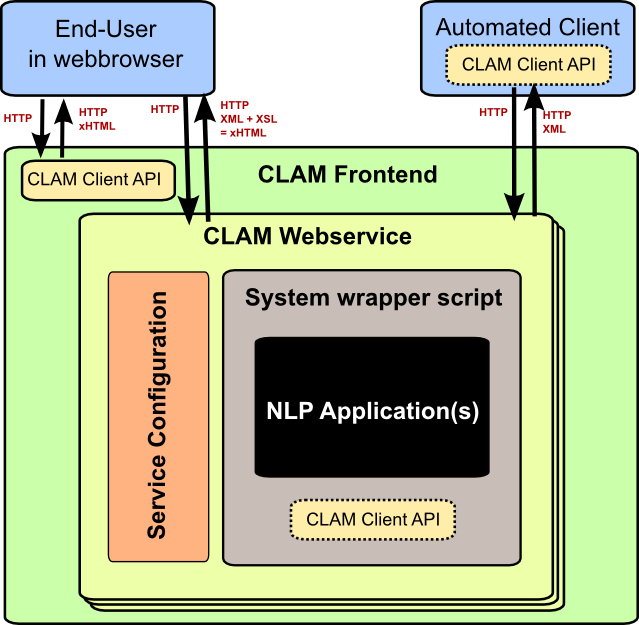
\includegraphics[width=130.0mm]{architecture.png}
\end{center}
\caption{The CLAM Architecture}
\label{fig:arch} 
\end{figure}

CLAM presents two different paradigms for wrapping your script or application.
The second is a new addition since CLAM 0.9.11 . You may use either or both at
the same time.

\begin{enumerate}
  \item \textbf{Project Paradigm} -- Users create projects, upload files with
    optional parameters to those projects, and subsequently start the project,
    optionally passing global parameters to the system. The system may run for
    a long time and may do batch-processing on multiple input files. 
  \item \textbf{Action Paradigm} -- This is a more limited, and simple
    remote-procedure call mechanism. Users interact in real-time with the service on
    specific URLs, passing parameters. Unlike the project paradigm, this is not
    suitable for complex operations on big-data.
\end{enumerate}

A CLAM webservice needs the following three components from the service developer:

\begin{enumerate}
\item A service configuration file;
\item A wrapper script for your command line application;
\item A command line application (your NLP tool)
\end{enumerate}

The wrapper script is not strictly mandatory if the command line application can be
directly invoked by CLAM. However, for more complex applications, writing a
wrapper script is recommended, as it offers more flexibility and
better integration, and allows you to keep the actual application
unmodified. The wrapper scripts can be seen as the ``glue'' between CLAM and
your application, taking care of any translation steps.

Note that wrapper scripts in the action paradigm are more constrained,  and
there may be multiple wrapper scripts for different actions.

\section{Beginning a new CLAM project}

You start a new CLAM project using the \texttt{clamnewproject} tool. The tool
generates all the necessary files, which you have to edit.  The tool takes one
argument: an identifier for your system. This identifier is for internal use,
possibly for use in URLs, and for use in filenames and may not contain any
spaces or other special characters. Mind that this ID is case sensitive, so it
is strongly recommended to keep it all lower case. Example:

{ \small
\begin{verbatim}
$ clamnewproject myfirstproject 
\end{verbatim}
}

The tool will create a directory named after the identifier, in which three
template files are created which are similarly named after the chosen
identifier. You are expected to edit the service configuration file, a Python
script, and one of the two system wrapper scripts (choose Python or Bash, or write
one from scratch in your favourite language). The scripts are heavily commented
to help you along, along with the documentation you are reading, this should
provide you with all knowledge necessary to make a webservice.

\begin{itemize}
\item \texttt{myfirstproject.py} - Service Configuration File
\item \texttt{myfirstproject\_wrapper.py} - System Wrapper Script in Python (this is recommended over the bash version for more complex webservices)
\item \texttt{myfirstproject\_wrapper.sh} - System Wrapper Script in Bash (only suggested for simple webservices)
\end{itemize}

Moreover, some scripts and sample configurations are generated:

\begin{itemize}
\item \texttt{startserver\_development.sh} - Start your webservice using the development server
\item \texttt{startserver\_production.sh} - Start your webservice using the production server using uwsgi. To use this you will need to configure your webservice (e.g. Apache or nginx).
\item \texttt{*.conf} - Sample configuration files for production environments using a Apache 2 or Nginx. Consult sections~\ref{sec:uwsgi} and~\ref{sec:uwsginginx} for details.
\end{itemize}

These template files need to be edited for your particular application.  They
are heavily commented to guide you. An \texttt{INSTRUCTIONS} file will be
created in your project directory, containing instructions on what files to
edit and how to start the clam service for your specific project. Starting your
webservice is as easy as running \texttt{startserver\_development.sh}, the
script will inform you to what URL to direct your browser once the webservice is running.

You can choose not to make use of one of the generated system wrapper scripts
and instead either write one from scratch in another language of your choice,
or directly let CLAM invoke your application. Moreover, a wrapper is intended
for the project paradigm, the action paradigm does not make use of it.

The next section will provide a detailed overview of the various ways to
configure the service configuration file, and the section thereafter will deal
with the system wrapper file.

\section{Service configuration}
\label{sec:serviceconfig}

The service configuration consists of a description of your NLP application, or
rather, a description of the system wrapper script that surrounds it. It
specifies what parameters the system can take, and what input and output
formats are expected under what circumstances. The service configuration is
itself a Python script, but knowledge of Python is not essential for you to be
able to make your own service configurations. 

It is assumed you are using the \texttt{clamnewproject} tool, which generates a
template service configuration you can edit. When reading this section, it may
help your understanding to inspect this file alongside.

One of the first things to configure is the root path (\texttt{ROOT}). All
projects will be confined to the \texttt{projects/} directory within this root
path, each project having its own subdirectory. When your NLP application or
wrapper script is launched, the current working directory will be set to this
project directory. Pre-installed corpora should be put in the \texttt{corpora/}
directory. The \texttt{ROOT} will be automatically created upon the first run.

\subsection{Server Administration}
\label{sec:sadmin}

The hostname and port of the webserver can be configured in the service
configuration file. Note that the hostname has to match exactly with what the
end-users will use. An attempt will be made to detect this automatically if no
hostname is specified. A mismatch in the name you define and the hostname the
user uses may result in unexpected behaviour. \footnote{Most likely, the XSLT
stylesheet will refuse to render the web application interface due to this
mismatch.}. CLAM comes with a built-in development webserver, started using the
\texttt{startserver\_development.sh} script in your project. 

When CLAM runs in a production environment using an existing webserver without
its own virtual host, it is often configured at a different URL rather than the
webserver root. In this case, the value of \texttt{URLPREFIX} should be
configured accordingly. If you want your webservice to run at
\url{http://yourhost.com/yourwebservice/} for instance, then the
\texttt{URLPREFIX} should be set to \texttt{yourwebservice}.

In order to keep server load manageable, three methods are configurable in the
service configuration file. First, you can set the variable
\texttt{REQUIREMEMORY} to the minimum amount of free memory that has to be
available (in megabytes, and not considering swap memory!). If not enough
memory is free, users will not be able to launch new processes, but will
receive an HTTP 500 error instead. Second, there is the \texttt{MAXLOADAVG}
variable; if the 5-minute load average exceeds this number, new processes will
also be rejected. Third, there is \texttt{MINDISKSPACE} and \texttt{DISK}. This
sets a constraint on the minimum amount of free disk space in megabytes on the
specified DISK (for example: \texttt{/dev/sda1}), which should be the disk
holding \texttt{ROOT}. If any of these values is set to zero, the checks are
disabled. Note though that this makes your system vulnerable to
denial-of-service attacks by possibly malicious users, especially if no user
authentication is configured!

Extra resource control is handled by the CLAM Dispatcher; a small program that
launches and monitors your wrapper script. In your service configuration file
you can configure the variable \texttt{DISPATCHER\_MAXRESMEM} and
\texttt{DISPATCHER\_MAXTIME}. The former is the maximum memory consumption of
your process, in megabytes. The latter is the maximum run-time of your process
in seconds. Programs that exceed this limit will be automatically aborted. The
dispatcher will check with a certain interval, configured in
\texttt{DISPATCHER\_POLLINTERVAL} (in seconds), if the limits have been
exceeded and will take the necessary action.  
  

If for some reason you do not want to make use of the web-based user interface
in CLAM, then you can disable it by setting \texttt{ENABLEWEBAPP = False}. If
you want to make the webservice available at a different URL than where the
webapplication is located, there is a small trick you can apply by setting
\texttt{WEBSERVICEGHOST} to a URL prefix that the webservice will be made
available on \emph{without} webapplication support. If you set for example
\texttt{WEBSERVICEGHOST = 'ws'}, then there will be an additional ``ghosted''
webservice without webapplication interface running on
\texttt{http://yourdomain.com/ws/}. This option is included to accommodate the
wish to apply two distinct authentication schemes outside of CLAM. 

CLAM offers a limited web-based administrative interface that allows you to
view what users and projects there are,  access their files, abort runs, and
delete projects. This interface can be accessed on the \texttt{/admin/} URL,
but requires that the logged-in user is in the list of \texttt{ADMINS} in the
service configuration file. The administrative interface itself does not offer
any means to adjust configuration options.

\subsection{User Authentication}

Being a RESTful webservice, user authentication proceeds over HTTP itself. CLAM
implements HTTP Digest Authentication \cite{HTTPAUTH} and OAuth2 \cite{OAUTH2}. HTTP Digest
Authentication, contrary to HTTP Basic Authentication, computes a hash of the
username and password client-side and transmits that hash, rather than a
plaintext password. User passwords are therefore only available to CLAM in
hashed form. User authentication is not mandatory, but for any world-accessible
environment it is most strongly recommended, for obvious security reasons.

A list of user accounts and passwords can be defined in \texttt{USERS} in the
service configuration file itself. This is a simple method allowing you to
quickly define users, but it is not a very scalable method. The \texttt{USERS}
variable is a dictionary of usernames mapped to an md5 hash computed on the
basis of the username, a string representing the security realm (by default the
system ID), and the password. Projects will only be accessible and visible to
their owners, unless no authentication is used at all, in which case everybody
can see all projects. An example of a configuration with plain text password,
converted on the fly to hashes, is found below:

{ \small
\begin{verbatim}
    USERS = {
        'bob': pwhash('bob', SYSTEM_ID, 'secret'), 
        'alice': pwhash('alice', SYSTEM_ID, 'secret2'),
    }
\end{verbatim}
}

However, computing hashes on the fly like in the above example is quite
insecure and not recommended. You should pre-compute the hashes and add these
instead:

{ \small
\begin{verbatim}
    USERS = {
        'bob': '6d72b6376858cf3c618c826fab1b0109',
        'alice': 'e445370f57e19a8bfa454404ba3892cc',
    }
\end{verbatim}
}

This pre-computation can be done in an interactive python session, executed from
the CLAM directory. Make sure to change \texttt{yourconfig} in the
example below to your actual service configuration file:

{ \small
\begin{verbatim}
$ python
>>> from clam.common.digestauth import pwhash
>>> import clam.config.yourconfig as settings
>>> pwhash('alice', settings.SYSTEM_ID, 'secret')
'e445370f57e19a8bfa454404ba3892cc'
\end{verbatim}
}

You can mark certain users as being administrators using the \texttt{ADMINS}
list. Administrators can see and modify all projects.


The ability to view and set parameters can be restricted to certain users. You
can use the extra parameter options \texttt{allowusers=} or \texttt{denyusers=}
to set this. See Section~\ref{sec:parameters}. A common use would be to define
one user to be the guest user, for instance the user named ``guest'', and set
\texttt{denyusers=['guest']} on the parameters you do not want the guest user
to use.

\subsubsection{MySQL backend}

Rather than using \texttt{USERS} to define a user database in your service
configuration file, a more sophisticated method is available using MySQL. The
configuration variable \texttt{USERS\_MYSQL} can be configured, instead of
\texttt{USERS}, to point to a table in a MySQL database somewhere; the fields
``username'' and ``password'' in this table will subsequently be used to
authenticate against. Custom field names are also possible. This approach
allows you to use existing MySQL-based user databases. The password field is
again a hashed password in the same fashion as in \texttt{USERS}, so it never
contains a plaintext password. \texttt{USERS\_MYSQL} is set as a Python
dictionary with the following configurable keys:

{ \small
\begin{verbatim}
    USERS_MYSQL = {
        'host': 'localhost',  #(default)
        'user': 'mysql_user',        
        'password': 'secret_mysql_password',
        'database': 'clamopener',
        'table': 'clamusers_clamusers',
        'userfield': 'username',      #(default)
        'passwordfield': 'password',  #(default)
    }
\end{verbatim}
}

\subsubsection{External authentication schemes}

Extra security may also be provided on a more global webserver level, rather
than in CLAM itself. For advanced service providers wanting to use external
authentication schemes, such as federated identity solutions, CLAM supports the
\texttt{PREAUTHHEADER} configuration directive, the value of which is a string
containing an HTTP header which CLAM may read to obtain the authenticated
username. This should be set by an authentication system \emph{prior} to
passing control to CLAM. An example of such a system is Shibboleth
\footnote{http://shibboleth.net}.  Multiple headers may be specified in
\texttt{PREAUTHHEADER}, using space as delimiter, effectively creating a
fallback chain. When \texttt{PREAUTHONLY} is set to \texttt{False} (default),
the ultimate fallback will be CLAM's built-in user system, unless this is set
to None. When such a scheme is used, proper care has to be taken to ensure that
the HTTP headers cannot be forged by end users themselves! If usernames that
come from external pre-authentication methods are different from those in the
internal \texttt{USERS} map (if used at all), an explicit mapping between
the two may be specified in the \texttt{PREAUTHMAPPING} dictionary. Note that
this pre-authentication mechanism never applies to the ``ghosted'' webservice,
if enabled through \texttt{WEBSERVICEGHOST}. Only the regular authentication
method is supported for the webservice ghost.

The example below shows an Apache configuration for a \emph{proxy server} or
\emph{entry server} that forwards to another server on which a CLAM service runs, mediated
through Shibboleth:

{ \small
\begin{verbatim}
   <Location /yourclamservice>
        AuthType shibboleth
        ShibRequireSession On
        ShibUseHeaders On
        require valid-user
        ProxyPass http://realserver/yourclamservice
        ProxyPassReverse http://realserver/yourclamservice
   </Location>
\end{verbatim}
}

The actual server, if it runs Apache, must always contain the directive \\
\texttt{WSGIPassAuthorization On}.

The CLAM service configuration file can in turn be restricted to accept \emph{only}
Shibboleth authenticated users using the following settings:

{ \small
\begin{verbatim}
PREAUTHHEADER = 'HTTP_EDUPERSONPRINCIPALNAME'
PREAUTHONLY = True
\end{verbatim}
}

Replace \texttt{HTTP\_EDUPERSONPRINCIPALNAME} with the proper HTTP header; this
variable name is just an example in a CLARIN-NL context.

\subsubsection{OAuth2}

CLAM also implements OAuth2 \cite{OAUTH2}, i.e. it acts as a client in the
OAuth2 Authorization framework. An external OAuth2 authorization provider is
responsible for authenticating you, using your user credentials to which CLAM
itself will never have access. Many OAuth2 providers exists; such as Google,
Facebook and Github, but you most likely want to use the OAuth2 provider of
your own institution. You will need to register your webservice with your
authentication provider, and obtain a \texttt{CLIENT\_ID} and
\texttt{CLIENT\_SECRET}, the latter should be kept strictly private! These go
into your service configuration file and we then enable OAuth as follows: 

{ \small
\begin{verbatim}
OAUTH = True
OAUTH_CLIENT_ID = "some_client_id"
OAUTH_CLIENT_SECRET = "donotsharewithanyone"
\end{verbatim}
}

Note that OAuth2 by definition requires HTTPS, therefore, it can not be used
with the built-in webserver but requires being embedded in a webserver such as
Apache2, with SSL support.

When the user approaches the CLAM webservice, he/she will need to pass a valid
access token. If none is passed, the user is instantly delegated to the OAuth2
authorization provider\footnote{CLAM responds with a HTTP 303 - See Other}.
The authorization provider makes available a URL for authentication and for
obtaining the final access token. These are configured as follows in the CLAM
service configuration file: 


{ \small
\begin{verbatim}
OAUTH_AUTH_URL= "https://yourprovider/oauth/authenticate"
OAUTH_TOKEN_URL "https://yourprovider/oauth/token"
\end{verbatim}
}

The authorization provider in turn redirects the user back to the CLAM
webservice, which in turn returns the access token to the client in its XML
response as follows. Note that there will just be this one tag without any
children.

{ \small
\begin{verbatim}
<clam xmlns:xlink="http://www.w3.org/1999/xlink" version="$version"
id="yourservice"
 name="yourservice" baseurl="https://yourservice.com/"
 oauth_access_token="1234567890">
</clam>
\end{verbatim}
}

Now any subsequent call to CLAM must pass this access token, otherwise you'd
simply be redirected to authenticate again. The client must thus explicitly call CLAM
again. Passing the access token can be done in two ways, the recommended way is
by sending the following HTTP header in your request, where the number is
replaced with the actual access token:

{ \small
\begin{verbatim}
Authentication: Bearer 1234567890
\end{verbatim}
}

The alternative way is by passing it along with the HTTP GET/POST request. This
is considered less secure as your browser may log it in its history, and the
server in its access logs. It can still not be intercepted, however, as it is
transmitted over HTTPS.

{ \small
\begin{verbatim}
https://yourservice.com/?oauth_access_token=1234567890
\end{verbatim}
}

Automated clients can avoid this method, but it is necessarily used by the
web-based interface. To mitigage security concerns, the access token you
receive is encrypted by CLAM and bound to your IP. The passphrase for token
encryption has to be configured through \texttt{OAUTH\_ENCRYPTIONSECRET} in
your secrive confifuration file. The web interface will furthermore explicitly
ask users to log out. Logging out is done by revoking the access token with the
authorization provider. For this to work, your authentication provider must
offer a revoke URL, as described in RFC7009\footnote{
\url{https://tools.ietf.org/html/rfc7009}}, which you configure in your service
configuration file as follows:

{ \small
\begin{verbatim}
OAUTH_REVOKE_URL = "https://yourprovider/oauth/revoke"
\end{verbatim}
}

If none is set, CLAM's logout procedure will simply instruct users to clear
their browser history and cache, which is clearly sub-optimal.

The only information CLAM needs from the authorization provider is a username.
The setting \texttt{OAUTH\_USERNAME\_FUNCTION} refers to a (Python) function
that obtains this from your resource provider after you have been
authenticated. It gets a single argument, the instance \texttt{oauthsession}
instance, and returns the username as a string.  The following example shows
how to implement this function for a resource provider that returns the
username in JSON format. This, however, is completely provider-specific so
you always have to write your own function! 

{ \small
\begin{verbatim}
def myprovider_username_function(oauthsession):
  r = oauthsession.get("https://yourprovider/user")
  d = json.loads(r.content)
  return d['username']

OAUTH_USERNAME_FUNCTION = myprovider_username_function
\end{verbatim}
}

Various providers require the system to specify scopes, indicating the
permissions the application requests from the resource provider. This can be
done using the \texttt{OAUTH\_SCOPE} directive in the service configuration
file, which takes a list of scopes, all of which are provider-specific. The
following example refers to the Google API:

{ \small
\begin{verbatim}
OAUTH_SCOPE = [
     "https://www.googleapis.com/auth/userinfo.email",
     "https://www.googleapis.com/auth/userinfo.profile"
]
\end{verbatim}
}

One of the problems with OAuth2 for automated clients is the authentication
step that often requires user intervention. CLAM redirects unauthenticated
users to the authorization provider. This is generally a website where the user
enters his username and password, but the means by which authentication
proceeds is not fixed by the OAuth2 specification. After authentication, the
site passes a one-time authorization code back to the user, with which the user
goes to CLAM to obtain the actual access token. This access token may be used
for a longer time, depending on the authorization provider.

This implies that automated clients accessing the CLAM service can not
authenticate in a generic fashion that is equal accross authorization
providers, there is again a provider-specific component here and CLAM clients
need to know how to communicate with the specific authorization provider.

At the moment, CLAM does not yet implement support for refresh tokens.

The unencrypted access token may be passed to the wrapper script if needed (has
to be explicitly configured), allowing the wrapper script or underlying system
to communicate with a resource provider on behalf of the user, through CLAM's
client\_id.

\subsection{Command Definition} \label{sec:command}

Central in the configuration file is the command that CLAM will execute. This
command should start the actual NLP application, or preferably a script wrapped
around it. Full shell syntax is supported. In addition there are some special
variables you can use that will be automatically set by CLAM. 

\begin{itemize}
\item \texttt{\$INPUTDIRECTORY} -- The absolute path to the input directory where all the input files from the user will be stored (possibly in subdirectories). This input directory is the \texttt{input/} subdirectory in the project directory.
\item \texttt{\$OUTPUTDIRECTORY} -- The absolute path to the output directory. Your system should output all of its files here, as otherwise they are not accessible through CLAM.  This output directory is the \texttt{output/} subdirectory in the project directory.
\item \texttt{\$STATUSFILE} -- The absolute path to a status file. Your system may write a short message to this status file, indicating the current status. This message will be displayed to the user in CLAM's interface. The status file contains a full log of all status messages, thus your system should write to this file in append mode. Each status message consists of one line terminated by a newline character. The line may contain three tab delimited elements that will be automatically detected: a percentage indicating the progress until completion (two digits with a \% sign), a Unix timestamp (a long number), and the status message itself (a UTF-8 string).
\item \texttt{\$PARAMETERS} -- This variable will contain all parameter flags
  and the parameter values that have been selected by the user. It is
  recommendedm however, to use \$DATAFILE instead of \$PARAMETERS.
\item \texttt{\$DATAFILE} -- The absolute path to the data file that CLAM outputs in the project directory. This data file, in CLAM XML format, contains all parameters along with their selected values. Furthermore it contains the inputformats and outputformats, and a listing of uploaded input files and/or pre-installed corpora. System wrapper scripts can read this file to obtain all necessary information, and as such this method is preferred over using \$PARAMETERS. If the system wrapper script is written in Python, the CLAM Data API can be used to read this file, requiring little effort on the part of the developer. 
\item \texttt{\$USERNAME} -- The username of the logged-in user.
\item \texttt{\$PROJECT} -- The ID of the project
\item \texttt{\$OAUTH\_ACCESS\_TOKEN} -- The unencrypted OAuth access token\footnote{As this is passed as a command line parameter, it may be exposed in the process list to other users on the machine CLAM is hosted on!}.
\end{itemize}


Make sure the actual command is an absolute path, or that the executable is in
the \texttt{\$PATH} of the user \texttt{clamservice.py} will run as. Upon
launch, the current working directory will be automatically set to the specific
project directory. Within this directory, there will be an \texttt{input/} and
\texttt{output/} directory, but use the full path as stored in
\texttt{\$INPUTDIRECTORY}/ and \texttt{\$OUTPUTDIRECTORY}/. All uploaded user
input will be in this input directory, and all output that users should be able
to view or download, should be in this output directory. Your wrapper script
and NLP tool are of course free to use any other locations on the filesystem
for whatever other purposes.


\subsection{Project Paradigm: Metadata, Profiles \& Parameters}

In order to explain how to build service configuration files for the tools you
want to make into webservices, we first need to clarify the project paradigm CLAM uses.
We shall start with a word about metadata. Metadata is data \emph{about}\/ your
data, i.e. data about your input and output files. Take the example of a plain
text file: metadata for such a file can be for example the character encoding
the text is in, and the language the text is written in. Such data is not
necessarily encoded within the file itself, as is also not the case in the
example of plain text files. CLAM therefore builds external metadata files for
each input and output file. These files contain all metadata of the files they
describe. These are stored in the CLAM Metadata XML format, a very simple and
straightforward format. \footnote{It is in essence a simple XML representation of
key--value pairs. These metadata files are named \texttt{.filename.METADATA},
in which filename is the name of the file it describes and resides in the very
same input/output directory.} Metadata simply consists of metadata fields
and associated values.

Metadata in CLAM is tied to a particular file format (such as plain text
format, CSV format, etc.). A format defines what kind of metadata it absolutely
needs, but usually still offers a lot of freedom for extra metadata fields to
the service provider, or even to the end user. 

When a user or automated client uploads a new input file, metadata is often not
available yet. The user or client is therefore asked to provide this. In the
webapplication a form is presented with all possible metadata parameters; the
system will take care of generating the metadata files according to the choices
made. If the service provider does not want to make use of any metadata
description at all, then that is of course an option as well, though this may
come at the cost of your service not providing enough information to interact
with others.

In a webservice it is important to define precisely what kind of input goes in,
and what kind of output goes out: this results in a deterministic and thus
predictable webservice. It is also necessary to define exactly how the output
metadata is based on the input metadata, if that is the case. These definitions
are made in so-called \emph{profiles}. A profile defines \emph{input templates}
and \emph{output templates}. The input templates and output template can be
seen as ``slots'' for certain filetypes and metadata. An analogy from childhood
memory may facilitate understanding this, as shown and explained in
Figure~\ref{fig:blokkendoos}.

\begin{figure}[h]
\begin{center}
\includegraphics[width=100.0mm]{blokkendoos.jpg}
\caption{Box and blocks analogy from childhood memory: the holes on one end
correspond to input templates, the holes on the other end correspond to output
templates. Imagine blocks going in through one and out through the other. The
blocks themselves correspond to input or output files \emph{with attached
metadata}. Profiles describe how one or more input blocks are transformed into
output blocks, which may differ in type and number. Granted, I am stretching the
analogy here; your childhood toy did not have this magic feature of course!}
\label{fig:blokkendoos} 
\end{center}
\end{figure}

A profile is thus a precise specification of what output files will be produced
given particular input files, and it specifies exactly how the metadata for the
outputfiles can be constructed given the metadata of the inputfiles. The
generation of metadata for output files is fully handled by CLAM, outside of
your wrapper script and NLP application.

Input templates are specified in part as a collection of parameters for which
the user/client is expected to choose a value in the predetermined range.
Output templates are specified as a collection of ``metafields'', which simply
assign a value, unassign a value, or copy a value from an input template or from
a global parameter. Through these templates, the actual metadata can be
constructed. Input templates and output templates always have a label
describing their function. Upon input, this provides the means for the user to
recognise and select the desired input template, and upon output, it allows the
user to easily recognise the type of output file. How all this is specified
exactly will be demonstrated in detail later.

In addition to input files and the associated metadata parameters, there is
another source of data input: global parameters. A webservice may define a set
of parameters that it takes. We will start by explaining this part in the next
section.


\subsection{Parameter Specification}
\label{sec:parameters}

The global parameters which an NLP application, or rather the wrapper script,
can take, are defined in the service configuration file. These parameters can
be subdivided into parameter groups, but these serve only presentational
purposes. 

%MAYBE TODO: CUSTOMPARAMETERS?
There are seven parameter types available, though custom types can be easily
added. \footnote{Use \texttt{common/parameters.py}} Each parameter type is a
Python class taking the following mandatory arguments:

\begin{enumerate}
\item \textbf{\texttt{id}} -- An id for internal use only.
\item \textbf{\texttt{name}} -- The name of this parameter; this will be shown to the user in the interface.
\item \textbf{\texttt{description}} -- A description of this parameter, meant for the end-user.
\end{enumerate}

The seven parameter types are:

\begin{itemize}
\item \textbf{\texttt{BooleanParameter}} -- A parameter that can only be turned on or off, represented in the interface by a checkbox. If it is turned on, the parameter flag is included in \texttt{\$PARAMETERS}, if it is turned off, it is not. If \texttt{reverse=True} is set, it will do the inverse.
\item \textbf{\texttt{IntegerParameter}} -- A parameter expecting an integer number. Use \texttt{minrange=}, and \texttt{maxrange=} to restrict the range if desired.
\item \textbf{\texttt{FloatParameter}} -- A parameter expecting a float number. Use \texttt{minrange=}, and \texttt{maxrange=} to restrict the range if desired.
\item \textbf{\texttt{StringParameter}} -- A parameter taking a string value. Use \texttt{maxlength=} if you want to restrict the maximum length.
\item \textbf{\texttt{TextParameter}} -- A parameter taking multiple lines of text. 
\item \textbf{\texttt{ChoiceParameter}} -- A multiple-choice parameter. The
  choices must be specified as a list of \texttt{(ID, label)} tuples, in which
  ID is the internal value, and label the text the user sees. For example,
  suppose a parameter with flag \texttt{-c} is defined.
  \texttt{choices=[('r','red'),('g','green'),('b', 'blue)]}, and the user
  selects ``green'', then  \texttt{-c g} will be added to \\
  \texttt{\$PARAMETERS}. The default choice can be set with \texttt{default=},
  and then the ID of the choice. If you want the user to be able to select
  multiple parameters, you can set the option \texttt{multi=True}. The IDs
  will be concatenated together in the parameter value. A delimiter (a comma by
  default) can be specified with \texttt{delimiter=}. If you do not use
  \texttt{multi=True}, but you do want all options to be visible in one view,
  you can set the option \texttt{showall=True}.
\item \textbf{\texttt{StaticParameter}} -- A parameter with a fixed immutable
  value. This may seem a bit of a contradiction, but it serves a purpose in
  forcing a global parameter or metadata parameter to have a specific non-variable value.
\end{itemize}

All parameters can take the following extra keyword arguments:

\begin{itemize}
\item \textbf{\texttt{paramflag}} -- The parameter flag. This flag will be
  added to \texttt{\$PARAMETERS} when the parameter is set. Consequently, it is
  mandatory if you use the \texttt{\$PARAMETERS} variable in your
  \texttt{COMMAND} definition. It is customary for parameter flags to consist
  of a hyphen and a letter or two hyphens and a string. Parameter flags could
  for example be formed like: \texttt{-p} ,\texttt{--pages},
  \texttt{--pages=}. There will be a space between the parameter flag and its
  value, unless it ends in a \texttt{=} sign or \texttt{nospace=True} is set.
  Multi-word string values will automatically be enclosed in quotation marks
  for the shell to correctly parse them. Technically, you are also allowed to
  specify an empty parameter flag, in which case only the value will be
  outputted as if it were an argument.
\item \textbf{\texttt{default}} -- Set a default value.
\item \textbf{\texttt{required}} -- Set to \texttt{True} to make this parameter required rather than optional.
\item \textbf{\texttt{require}} -- Set this to a list of parameter IDs. If this parameter is set, so must all others in this list. If not, an error will be returned.
\item \textbf{\texttt{forbid}} -- Set this to a list of parameter IDs. If this parameter is set, none of the others in the list may be set.  If not, an error will be returned.
\item \textbf{\texttt{allowusers}} -- Allow only the specified lists of usernames to see and set this parameter. If unset, all users will have access. You can decide whether to use this option or \texttt{denyusers}, or to allow access for all.
\item \textbf{\texttt{denyusers}} -- Disallow the specified lists of usernames to see and set this parameter. If unset, no users are blocked from having access. You can decide whether to use this option or \texttt{allowusers}, or to allow access for all.
\end{itemize}

The following example defines a boolean parameter with a parameter flag:

{\small
\begin{verbatim}
BooleanParameter(
  id='createlexicon',
  name='Create Lexicon',
  description='Generate a separate overall lexicon?',
  paramflag='-l'
)
\end{verbatim}
}

Thus, if this parameter is set, the invoked command will have \texttt{\$PARAMETERS} set to \texttt{-l 1} (plus any additional parameters).

\subsection{Profile specification}

Multiple profiles may be specified, and all profiles are always assumed to be
independent of each other. Dependencies should be together in one profile, as
each profile describes how a certain type of input file is transformed into a
certain type of output file. For each profile, you need to define input
templates and output templates. All matching profiles are assumed to be
delivered as promised. A profile matches if all input files according to the
input templates of that profile are provided and if it generates output. If no
input templates have been defined at all for a profile, then it will match as
well, to allow for the option of producing output files that are not dependent
on input files. A profile is allowed to mismatch, but if none of the profiles
match, the system will produce an error, as it cannot perform any actions. 

The profile specification skeleton looks as follows. Note that there may be
multiple input templates and/or multiple output templates:

{\small
\begin{verbatim}
PROFILES = [ 
    Profile( InputTemplate(...), OutputTemplate(...) ) 
]
\end{verbatim}
}


The definition for \texttt{InputTemplate} takes three mandatory arguments:

\begin{enumerate}[leftmargin=5mm]
\item \texttt{id} -- An ID for the InputTemplate. This will be used internally and by automated clients.
\item \texttt{format} -- This points to a Format class, indicating the kind of format that this input template accepts. Formats are defined in \texttt{clam/common/formats.py}. Custom formats can be added there. Custom format classes can also be defined in the service configuration itself, after which you need to add these classes to the \texttt{CUSTOM\_FORMATS} list.
\item \texttt{label} -- A human readable label for the input template. This is how it will be known to users in the web application and displayed in its selection menus.
\end{enumerate}

After the three mandatory arguments, you may specify any of the Parameter types
to indicate the accepted/required metadata for the particular input templates.
Use any of the types from Section~\ref{sec:parameters}. We will come to an
example of this soon. 

After specifying any such parameters, there are some possible keyword arguments:

\begin{enumerate}[leftmargin=5mm]
\item \texttt{unique} -- Set to \texttt{True} or \texttt{False}; this indicates whether the input template may be used only once or multiple times. \texttt{unique=True} is the default if not specified.
\item \texttt{multi} -- The logical inverse of the above; you can whichever you prefer. \texttt{multi=False} is the default if not specified.
\item \texttt{filename} -- Files uploaded through this input template will
  receive this filename (regardless of how the original file on the client is
  called). If you set \texttt{multi=True} or its alias \texttt{unique=False},
  insert the variable \texttt{\$SEQNR} into the filename, which will be
  replaced by a number in sequence. After all, we cannot have multiple files
  with the same name. As explained in Section~\ref{sec:filenamevariables}, you
  can also use any of the metadata parameters as variable in the filename.
\item \texttt{extension} -- Files uploaded through this input template are
  expected to have this extension, but can have any filename. Here it
  does not matter whether you specify the extension with or without the
  prefixing period. Note that in the web application, the extension is appended
  automatically regardless of the filename of the source file. Automated
  clients do must take care to submit files with the proper extension right away. 
\item \texttt{acceptarchive} -- This is a boolean which can be set to True if
  you want to accept the upload of archives. Uploaded archives will be
  automatically unpacked. It is a method to instantly upload multiple files
  \emph{for the same input template}. The file must be in zip, tar.gz or
  tar.bz2 format. The files within the archive will be
  renamed according to the input template's specifications if necessary. Using
  this option implies that the exact same metadata will be associated with all
  uploaded files! This option can only be used in combination with
  \texttt{multi=True}. Note that archives can only be uploaded when all files
  therein fit the same input template!
\end{enumerate}


Take a look at the following example of an input template for plaintext
documents for an automatic translation system, illustrating of all the above:

{\small
\begin{verbatim}
InputTemplate('maininput', PlainTextFormat,
  "Translator input: Plain-text document",  
  StaticParameter(
    id='encoding',name='Encoding',
    description='The character encoding of the file', 
    value='utf-8'
  ),  
  ChoiceParameter(
    id='language',name='Language',
    description='The language the text is in', 
    choices=[('en','English'),('nl','Dutch'),('fr','French')]),
  ),      
  extension='.txt',
  multi=True
)
\end{verbatim}
}


For \texttt{OutputTemplate}, the syntax is similar. It takes the three
mandatory arguments \emph{id}, \emph{format} and \emph{label}, and it also
takes the four keyword arguments laid out above. If no explicit filename has
been specified for an output template, then it needs to find out what name the
output filename will get from another source. This other source is the input
template that acts as the \emph{parent}. The output template will thus inherit
the filename from the input template that is its parent. In this way, the user
may upload a particular file, and get that very same file back with the same
name. If you specify \texttt{extension}, it will append an extra extension to
this inherited filename. Prior to appending an extension, you may often want to
remove an existing extension; you can do that with the \texttt{removeextension}
attribute. 
As there may be multiple input templates, it is not always clear what input
template is the parent. The system will automatically select the \emph{first}
defined input template with the same value for unique/multi the output template
has. If this is not what you want, you can explicitly set a parent using the
\texttt{parent} keyword, which takes the value of the input template's ID.

Whereas for \texttt{InputTemplate} you can specify various parameter types,
output templates work differently. Output templates define what metadata fields
(metafields for short) they want to set with what values, and from where to get
these values. In some situations the output file is an extension of the input
file, and you want it to inherit the metadata from the input file. Set
\texttt{copymetadata=True} to accomplish this: now all metadata will be
inherited from the parent, but you can still make modifications.

To set (or unset) particular metadata fields you specify so-called ``metafield
actors''. Each metafield actor sets or unsets a particular metadata attribute.
There are four different types of metafield actors:

\begin{itemize}
\item \texttt{SetMetaField(\emph{key},\emph{value})} -- Set metafield \emph{key} to the specified value.
\item \texttt{UnsetMetaField(\emph{key}\emph{[,value]})} -- If a value is
  specified: Unset this metafield if it has the specified value. If no value is
  specified: Unset the metafield regardless of value. This only makes sense if
  you set \\ \texttt{copymetadata=True}.
\item \texttt{CopyMetaField(\emph{key}, \emph{inputtemplate.key})} -- Copy
  metadata from one of the input template's metadata. Here \emph{inputtemplate}
  is the ID of one of the input templates in the profile, and the \emph{key}
  part is the metadata field to copy. This allows you to combine metadata from
  multiple input sources into your output metadata.
\item \texttt{ParameterMetaField(\emph{key}, \emph{parameter$-$id})} -- Get the value for this metadata field from a global parameter with the specified ID.
\end{itemize}

Take a look at the following example for a fictitious automatic translation
system, translating to Esperanto. If an input file \texttt{x.txt} is uploaded,
the output file will be named \texttt{x.translation}.

{\small
\begin{verbatim}
OutputTemplate('translationoutput', PlainTextFormat,
    "Translator output: Plain-text document",  
    CopyMetaField('encoding','maininput.encoding')
    SetMetaField('language','eo'),
    removeextension='.txt',
    extension='.translation',
    multi=True
)
\end{verbatim}
}

Putting it all together, we obtain the following profile definition describing
a fictitious machine translation system from English, Dutch or French to
Esperanto, where the system accepts and produces UTF-8 encoded plain-text
files.

{\small
\begin{verbatim}
PROFILES = [ 
  Profile( 
    InputTemplate('maininput', PlainTextFormat,
     "Translator input (Plain-text document)",  
      StaticParameter(
       id='encoding',name='Encoding',
       description='The character encoding of the file', 
       value='utf-8'
      ),  
      ChoiceParameter(
       id='language',name='Language',
       description='The language the text is in', 
       choices=[('en','English'),('nl','Dutch'),('fr','French')]
      ),
      extension='.txt',
      multi=True
    ), 
    OutputTemplate('translationoutput', PlainTextFormat,
      "Esperanto translation (Plain-text document)",  
      CopyMetaField('encoding','maininput.encoding')
      SetMetaField('language','eo'),
      removeextension='.txt',
      extension='.translation',
      multi=True
    )    
  )
]
\end{verbatim}
}


\subsection{Control over filenames}
\label{sec:filenamevariables}

There are several ways of controlling the way input and output files within a
profile are named. As illustrated in the previous section, each output template
has an input template as its parent, from which it inherits the filename if no
explicit filename is specified. This is a very important aspect that has to be
considered when building your profiles. By default, if no \texttt{filename=}, \texttt{extension=} or
\texttt{removeextension=} is specified for an output template, it will use the
same filename as the parent input template. If \texttt{filename=} and
\texttt{extension=} are not specified for the Input Template, then the file the
user uploads will simply maintain the very same name as it is uploaded with. If
\texttt{extension=} is specified, the input file is required to have the
specified extension, the web application and CLAM Client API takes care of this
automatically if this is not the case.

In a previous section, we mentioned the use of the variable \texttt{\$SEQNR}
that will insert a number in the filename when the input template or output template is in
multi-mode. In addition to this, other variables can also be used. Here is an
overview:

\begin{itemize}
\item \texttt{\$SEQNR} - The sequence number of the file. Valid only if \texttt{unique=True} or \texttt{multi=False}.
\item \texttt{\$PROJECT} - The ID of the project.
\item \texttt{\$INPUTFILENAME} - The filename of the associated input file. Valid only in Output Templates.
\item \texttt{\$INPUTSTRIPPEDFILENAME} - The filename of the associated input file without any extensions. Valid only in Output Templates.
\item \texttt{\$INPUTEXTENSION} - The extension of the associated input file (without the initial period). Valid only in Output Templates.
\end{itemize} 

Other than these pre-defined variables by CLAM, you can use
any of the metadata parameters as variables in the filename, for input
templates only. To this end, use a
dollar sign followed by the ID of the parameter in the filename specification.
For Output Templates, you can use metafield IDs or global parameter IDs (in
that order of priority) in the same way. This syntax is valid in both
\texttt{filename=} and \texttt{extension=}.

The following example illustrates a translation system that encodes the
character encoding and language in the filename itself. Note also the use of
the special variable \texttt{\$SEQNR}, which assigns a sequence number as the
templates are both in multi mode.

{\small
\begin{verbatim}
PROFILES = [ 
  Profile( 
    InputTemplate('maininput', PlainTextFormat,
      "Translator input (Plain-text document)",  
      StaticParameter(
       id='encoding',name='Encoding',
       description='The character encoding of the file', 
       value='utf-8'
      ),  
      ChoiceParameter(
       id='language',name='Language',
       description='The language the text is in', 
       choices=[('en','English'),('nl','Dutch'),('fr','French')]
      ),
      filename='input$SEQNR.$language.$encoding.txt'
      multi=True
    ), 
    OutputTemplate('translationoutput', PlainTextFormat,
      "Esperanto translation (Plain-text document)",  
      CopyMetaField('encoding','maininput.encoding')
      SetMetaField('language','eo'),
      filename='output$SEQNR.$language.$encoding.txt'
      multi=True
    )    
  )
]
\end{verbatim}
}

In addition to variables that refer to global or local parameters. There are some additional variables set by CLAM which you can use:

\begin{itemize}
\item \texttt{\$PROJECT} - Is set to the project ID.
\item \texttt{\$INPUTFILE} - Is set to the project ID.
\end{itemize}



\subsection{Parameter Conditions}

It is not always possible to define all output templates straight away.
Sometimes output templates are dependent on certain global parameters. For
example, given a global parameter that toggles the generation of a lexicon, you
want to include only the output template that describes this lexicon, if the
parameter is enabled. CLAM offers a solution for such situations using the
\texttt{ParameterCondition} directive.

Assume you have the following \emph{global} parameter:

{ \small
\begin{verbatim}
BooleanParameter(
  id='createlexicon',name='Create Lexicon',
  description='Create lexicon files', 
)
\end{verbatim}
}

We can then turn an output template into an output template conditional on this parameter using the following construction:

{ \small
\begin{verbatim}
  ParameterCondition(createlexicon=True, 
    then=OutputTemplate('lexiconoutput', PlainTextFormat,
      "Lexicon (Plain-text document)",  
      unique=True
    ) 
  )
\end{verbatim}
}

The first argument of ParameterCondition is the condition. Here you use the ID
of the parameter and the value you want to check against. The above example
illustrates an equality comparison, but other comparisons are also possible. We
list them all here:

\begin{itemize}
\item \texttt{\emph{ID}$=$\emph{value}} -- Equality; matches if the global parameter with the specified ID has the specified value.
\item \texttt{\emph{ID}\_equals$=$\emph{value}} -- Same as above, the above is an alias.
\item \texttt{\emph{ID}\_notequals$=$\emph{value}} -- The reverse of the above, matches if the value is \emph{not equal}
\item \texttt{\emph{ID}\_lessthan$=$\emph{number}} -- Matches if the parameter with the specified ID is less than the specified number
\item \texttt{\emph{ID}\_greaterthan$=$\emph{number}} -- Matches if the parameter with the specified ID is greater tha then specified number
\item \texttt{\emph{ID}\_lessequalthan$=$\emph{number}} -- Matches if the parameter with the specified ID is equal or less than the specified number
\item \texttt{\emph{ID}\_greaterequalthan$=$\emph{number}} -- Matches if the parameter with the specified ID is equal or greater than the specified number
\end{itemize}

After the condition you specify \texttt{then=} and optionally also
\texttt{else=}, and then you specify an \texttt{OutputTemplate} or yet another
\texttt{ParameterCondition}---they can be nested at will.

Parameter conditions cannot only be used for output templates, but also
for metafield actors, inside the output template specification. In other
words, you can make metadata fields conditional on global parameters.

Parameter conditions cannot be used for input templates, for the simple
reason that in CLAM the parameters are set after the input files are uploaded.
However, input templates can be \emph{optional}, by setting
\texttt{optional=True}. This means that providing such input files is optional.
This also implies that any output templates that have this optional input
template as a parent are also conditional on the presence of those input files.

%TODO LATER: Provide example?

\subsection{Converters}

Users do not always have their files in the format you desire as input, and
asking users to convert their data may be problematic. Similarly, users may not
always like the output format you offer. CLAM therefore introduces a converter
framework that can do two things:

\begin{enumerate}
\item Convert input files from auxiliary formats to your desired format, upon upload;
\item Convert output files from your output format to auxiliary formats.
\end{enumerate}

A converter, using the above-mentioned class names, can be included in input
templates (for situation 1), and in output templates (for situation 2). Include
them directly after any Parameter fields or Metafield actors.

It is important to note that the converters convert only the files themselves
and not the associated metadata. This implies that these converters are
intended primarily for end users and not as much for automated clients.

For most purposes, you will need to write your own converters. These are to be
implemented in \texttt{clam/common/converters.py}. Some converters however will
be provided out of the box. Note that the actual conversion will be performed
by 3rd party software in most cases.

\begin{itemize}
\item \texttt{MSWordConverter} -- Convert MS Word files to plain text. This
  converter uses the external tool \texttt{catdoc} by default.
  \footnote{\url{http://www.wagner.pp.ru/~vitus/software/catdoc/}}
\item \texttt{PDFConverter} -- Convert PDF to plain text. This converter uses
  the external tool \texttt{pdftohtml} by default. \footnote{\url{http://pdftohtml.sourceforge.net/}}
\item \texttt{CharEncodingConverter} -- Convert between plain text files in
  different character encodings.
\end{itemize}

Note that specific converters take specific parameters; consult the API reference for details.

%TODO LATER: Include examples?

\subsection{Viewers}

Viewers are intended for human end users, and enable visualisation of a
particular file format. CLAM offers a viewer framework that enables you to
write viewers for your format. Viewers may either be written within the CLAM
framework, using Python, but they can also be external (non-CLAM) webservices,
hosted elsewhere. Several simple viewers for some formats are provided already;
these are defined in \texttt{viewers.py}.

Viewers can be included in output templates. Include them directly after any
metafield actors.


The below example illustrates the use of the viewer
\texttt{SimpleTableViewer}, capable of showing CSV files:

{ \small
\begin{verbatim}
OutputTemplate('freqlist',CSVFormat,"Frequency list",
    SimpleTableViewer(),
    SetMetaField('encoding','utf-8'),
    extension='.patterns.csv',
)
\end{verbatim}
}

\subsection{Working with pre-installed data}

Rather than letting users upload files, CLAM also offers the possibility of
pre-installing input data on the server. This feature is ideally suited for
dealing with data for a demo, or for offering a selection of pre-installed
corpora that are too big to transfer over a network. Furthermore, pre-installed
data is also suited in situations where you want the user to be able to choose
from several pre-installed resources, such as lexicons, grammars, etc., instead
of having to upload files they may not have available.

Pre-installed data sources are called ``input sources'' in CLAM, not to be
confused with input templates. Input sources can be specified either in an
input template, or more globally. 

Take a look at the following example:

{ \small
\begin{verbatim}
InputTemplate('lexicon', PlainTextFormat,"Input Lexicon", 
   StaticParameter(id='encoding',name='Encoding',
       description='Character encoding',
       value='utf-8'),
   ChoiceParameter(id='language',name='Language',
       description='The language the text is in', 
       choices=[('en','English'),('nl','Dutch'),('fr','French')]),
   InputSource(id='lexiconA', label="Lexicon A",
    path="/path/to/lexiconA.txt", 
    metadata=PlainTextFormat(None, encoding='utf-8',language='en')
   ),
   InputSource(id='lexiconB', label="Lexicon B",
    path="/path/to/lexiconB.txt", 
    metadata=PlainTextFormat(None, encoding='utf-8',language='en')
   ),
   onlyinputsource=False
)            
\end{verbatim}
}

This defines an input template for some kind of lexicon, with two pre-defined
input sources: ``lexicon A'' and ``lexicon B''. The user can choose between
these, or alternatively upload a lexicon of his own. If, however,
\texttt{onlyinputsource} is set to \texttt{True}, then the user is forced to
choose only from the input sources, and cannot upload his own version. 

Metadata can be provided either in the inputsource configuration, or by simply
adding a CLAM metadata file alongside the actual file. For the file
\path{/path/to/lexiconA.txt}, the metadata file would be
\path{/path/to/.lexiconA.txt.METADATA} (note the initial period; metadata
files are hidden). 

Input sources can also be defined globally, and correspond to multiple files,
i.e. they point to a directory containing multiple files instead of pointing to
a single file. Let us take the example of a spelling correction demo, in which
a test set consisting out of many text documents is the input source:

{ \small
\begin{verbatim}
INPUTSOURCES = [
    InputSource(id='demotexts', label="Demo texts",
        path="/path/to/demotextdir/", 
        metadata=PlainTextFormat(None, encoding='utf-8',
                 language='en'),
        inputtemplate='maininput',
       ),
]
\end{verbatim}
}

In these cases, it is essential to set the \texttt{inputtemplate=} parameter.
All files in the directory must be formatted according to this input template.
Adding input sources for multiple input templates is done by simply defining
multiple input sources. %The user may always select from as many or few input
%sources as he wants.

\subsection{Multiple profiles, identical input templates}

It is possible and sometimes necessary to define more than one profile. Recall
that each profile defines what output will be generated given what input, and
how the metadata is translated. Multiple profiles come into the picture as soon
as you have a disjunction of possible inputs. Imagine a spelling check system
that can take either plain text as input, or a kind of XML file. In this
situation you have two profiles; one for the plain-text variant, and one for
the XML variant. 

Now suppose there is another kind of mandatory input, a lexicon against which
spell checking occurs, that is relevant for \emph{both} profiles, and exactly
the same for both profiles. In such circumstances, you could simply respecify
the full input template, with the same ID as in the other profile. The most
elegant solution however, is to instantiate the input template in a variable,
prior to the profile definition, and then use this variable in both profiles.


\subsection{Customising the web application}

The CLAM web application offers a single uniform interface for all kinds of
services. However, a certain degree of customisation is possible. One thing you
may want is to include more HTML text on the pages, possibly enriched with
images and hyperlinks to external sites. It is an ideal way to add extra
instructions for your users. You may do so using the following variables in the
service configuration file:


\begin{itemize}
\item \texttt{CUSTOMHTML\_INDEX} - This text will be included in the index view, the overview of all projects.
\item \texttt{CUSTOMHTML\_PROJECTSTART} - This text will be included in the project view where the user can upload files and select parameters.
\item \texttt{CUSTOMHTML\_PROJECTDONE} - This text will be included in the project view when the project is done and output is ready to be viewed/downloaded.
\end{itemize}

As the HTML text will be embedded on the fly, take care \emph{not} to include
any headers. Only tags that go within the HTML \texttt{body} are permitted!
Always use the utf-8 encoding and well-formed xhtml syntax.

A second kind of customisation is customisation of the style, which can be
achieved by creating new CSS themes. CLAM gets shipped with the default
``classic'' style (which did receive a significant overhaul in CLAM 0.9). Copy,
rename and adapt \texttt{style/classic.css} to create your own style. And set
\texttt{STYLE} accordingly in your service configuration file.

In your service configuration file you can set a variable
\texttt{INTERFACEOPTIONS}; this string is a space-separated list in which you
can use the following directives to customise certain aspects of the
web-interface:

\begin{itemize}
\item \texttt{simpleupload} -- Use the simple uploader instead of the more advanced javascript-based. The simple uploader does not support multiple files but does provide full HTTP Digest Security whereas the default and more advanced uploader relies on a less sophisticated security mechanism.
\item \texttt{simplepolling} -- Uses a simpler polling mechanism in the stage
  in which CLAM awaits the completion of a process. This method simply
  refreshes the page periodically, while the default method is asynchronous but relies on a less sophisticated security mechanism. 
\item \texttt{secureonly} -- Equals to \texttt{simpleupload} and \texttt{simplepolling}, forcing only methods that fully support HTTP Digest Authentication.
\item \texttt{disablefileupload} -- Disables the file uploader in the interface (do note that this is merely cosmetic and not a security mechanism, the RESTful webservice API will continue to support file uploads).
\item \texttt{inputfromweb} -- Enables downloading an input file from the web (do note that this is merely cosmetic and not a security mechanism, the RESTUL webservice API always supports this regardless of visibility in the interface).
\item \texttt{disableliveinput} -- Disables adding input through the live in-browser editor. 
\item \texttt{preselectinputtemplate} -- Pre-select the first defined input template as default inputtemplate.
\end{itemize}



\subsection{Actions}

Since CLAM 0.9.11, a simple remote procedure call mechanism is available in
addition to the more elaborate project paradigm. 

This action paradigm allows you to specify \emph{actions}, each action allows
you to tie a URL to a script or Python function, and may take a number of
parameters you explicitly specify. Each action is strictly independent of other
actions, and complete separate of the projects, and by extension also of any
files within projects and any profiles. Unlike projects, which may run over a
long time period and are suited for batch processing, actions are intended for
real-time communication. Typically they should return an answer in at most a
couple of seconds.

Actions are specified in the service configuration file in the \texttt{ACTIONS}
list. Consider the following example:


{ \small
\begin{verbatim}
ACTIONS = [
  Action(id='multiply',name="Multiplier",
  description="Multiply two
  numbers",command="/path/to/multiply.sh $PARAMETERS",
  mimetype="text/plain",
  parameters=[
    IntegerParameter(id='x',name="Value 1"),
    IntegerParameter(id='y',name="Value 2"),
  ])
]
\end{verbatim}
}

The ID of the action determines on what URL it listens. In this case the URL
will be \texttt{/actions/multiply/}, relative to the root of your service. The
name and display are for presentational purposes in the interface.

Actions will show in the web-application interface on the index page.

In this example, we specify two parameters, they will be passed \emph{in the
order they are defined} to the script. The command to be called is configured
analagous to \texttt{COMMAND}, but only a subset of the variables are
supported. The most prominent is the \texttt{\$PARAMETERS} variable. Note that
you can set \texttt{paramflag} on the parameters to pass them with an option
flag. String parameters with spaces will work without problem\footnote{Do note that
shells have a maximum length of all parameters combined}. Actions do not have
the notion of the CLAM XML datafile that wrapper scripts in the project
paradigm can use, so passing command-line parameters is the only way here.

It may, however, not even be necessary to invoke an external script. Actions
support calling Python functions directly. Consider the following trivial Python
function for multiplication:

{ \small
\begin{verbatim}
def multiply(a,b):
  return a * b
\end{verbatim}
}

You can define functions in the service configuration file itself, or import it
from elsewhere. We can now use this as an action directly:

{ \small
\begin{verbatim}
ACTIONS = [
  Action(id='multiply',name="Multiplier",
  description="Multiply two numbers",
  function=multiply,mimetype="text/plain"
  parameters=[
    IntegerParameter(id='x',name="Value 1"),
    IntegerParameter(id='y',name="Value 2"),
  ])
]
\end{verbatim}
}

Again, the parameters are passed in the order they are specified, irregardless
of their names. A mismatch in parameters will result in an error as soon as you
try to use the action. All parameters will always be validated prior to calling the
script or function.

When an action completes, the standard output of the script or the return
value\footnote{Will be serialised to a string automatically by CLAM, assuming
this is possible} of the function is returned to the user directly (as HTTP 200) and as-is.
It is therefore important to specify what MIME type the user can expect, the
default is \texttt{text/plain}, but for many applications \texttt{text/html}, \texttt{text/xml} or
\texttt{application/json} may be more appropriate.

By default, actions listen to both GET and POST requests. You may constrain it
explicitly by specifying \texttt{method="GET"} or \texttt{method="POST"}.

When a script is called, CLAM looks at its return code to determine whether
execution was successful ($0$). If not, CLAM will return the standard error
output in a ``HTTP 500 -- Internal Server Error'' reply. If define your own
errors and return standard \emph{output} in an HTTP 403 reply, use return code
$3$; for standard output in an HTTP 404 reply, use return code $4$. These are just defaults, all return
codes are configurable through the keyword arguments \texttt{returncodes200},
\texttt{returncodes403}, \texttt{returncodes404}, each being a list of
integers.

When using Python functions, exceptions will be caught and returned to the
end-user in a HTTP 500 reply (without traceback). For custom replies, Python
functions may raise any instance of \texttt{web.webapi.HTTPError}.

If you enabled an authentication mechanism, as is recommended, it automatically
applies to all actions. It is, however, possible to exempt certain actions from
needing authentication, allowing them to serve any user anonymously. To do so, add
the keyword argument \texttt{allowanonymous=True} to the configuration of the
action. 

If you want to use only actions and disable the project paradigm
entirely, set the following in your service configuration file:

{ \small
\begin{verbatim}
COMMAND = None
PROFILES = []
PARAMETERS = []
\end{verbatim}
}


\section{Wrapper script}

Service providers are encouraged to write a wrapper script that acts as the
glue between CLAM and the NLP Application(s). CLAM will execute the wrapper
script, and the wrapper script will in turn invoke the actual NLP
Application(s). Using a wrapper script offers more flexibility than letting
CLAM directly invoke the NLP Application, and allows the NLP Application itself
to be totally independent of CLAM. 

The wrapper script takes the arguments as specified in \texttt{COMMAND} in the
service configuration file; see Section~\ref{sec:command}. There are some
important things to take into account:

\begin{itemize}
\item All user-provided input has to be read from the specified input directory. A full listing of this input will be provided in the \texttt{clam.xml} data file. If you choose not to use this, but use \texttt{\$PARAMETERS} instead, then you must take care that your application can identify the file formats by filename, extension or otherwise.
\item All user-viewable output must be put in the specified output directory. Output files must be generated in accordance with the profiles that describe this generation. 
\item The wrapper should periodically output a small status message to
  \texttt{\$STATUSFILE}. While this is not mandatory, it offers valuable feedback to the user on the state of the system. 
\item The wrapper script is always started with the current working directory set to the selected project directory.
\item Wrapper scripts often invoke the actual application using some kind of
  \texttt{system()} call. Take care never to pass unvalidated user-input to the shell! This makes you vulnerable
  for code injection attacks. The CLAM Data API offers the function
  \texttt{clam.common.data.shellsafe()} to help protect you.
\end{itemize}

The wrapper script can be written in any language. Python developers will have
the big advantage that they can directly tie into the CLAM Data API, which
handles things such as reading the \texttt{clam.xml} data file, makes all
parameters and input files (with metadata) directly accessible, and offers a
function to protect your variables against code injection when passing them to
the shell.

If you used \texttt{clamnewproject} to begin your new clam service, then an example
wrapper script will have been created for you, using the CLAM Data API.

\subsection{CLAM Data API}

The key function of CLAM Data API is parsing the CLAM XML Data file that the
clam webservice uses to communicate with clients. This data is parsed and all
its components are made available in an instance of a CLAMData class.

Suppose your wrapper script is called with the following command definition:

{\footnotesize
\begin{verbatim}
COMMAND = "/path/to/wrapperscript.py $DATAFILE $STATUSFILE $OUTPUTDIRECTORY" 
\end{verbatim}}


Your wrapper scripts then typically starts in the following fashion:


{ \small
\begin{verbatim}
import sys
import clam.common.data

datafile = sys.argv[1]
statusfile = sys.argv[2]
outputdir = sys.argv[3]

clamdata = clam.common.data.getclamdata(datafile)
\end{verbatim}
}

The first statements parse the command line arguments. The last statement
returns a \texttt{CLAMData} instance, which contains all data your wrapper might need,
representing the state of the project and all user input.

For an extensive overview of the \texttt{CLAMData} class, we refer to the CLAM
Data API Documentation at \url{http://packages.python.org/CLAM}. It is highly
recommended to read this when your wrapper is using the CLAM Data API. A few of the
variables available are:

\begin{itemize}
\item \texttt{clamdata.system\_id}
\item \texttt{clamdata.project}
\item \texttt{clamdata.user}
\item \texttt{clamdata.status}
\item \texttt{clamdata.parameters}
\item \texttt{clamdata.input}
\end{itemize}


Any global parameters are available from the \texttt{clamdata} instance, by
using it like a Python dictionary, where the keys correspond to the Parameter ID:

{ \small
\begin{verbatim}
parameter = clamdata['parameter_id']
\end{verbatim}
}

The CLAM API also has facilities to use a status file to relay progress
feedback to the web-interface. Using it is as simple as importing the library
and writing messages at strategic points during your program's execution:

{ \small
\begin{verbatim}
import clam.common.status
clam.common.status.write(statusfile, "We are running!")
\end{verbatim}
}

Progress can also be expressed through an additional completion parameter,
holding a value between $0$ and $1$. The web-application will show a progress bar if
such information is provided:

{ \small
\begin{verbatim}
clam.common.status.write(statusfile, 
     "We're half way there! Hang on!", 0.5)
\end{verbatim}
}

If you have a specific input file you want to grab, you may obtain it from your
\texttt{clamdata} instance by inputtemplate:

{ \small
\begin{verbatim}
inputfile = clamdata.inputfile('some-inputtemplate-id')
inputfilepath = str(inputfile) 
\end{verbatim}
}

The variable \texttt{inputfilepath} in the above example will contain the full
path to the file that was uploaded by the user for the specified input
template. 

Once you have a file, you can easily obtain any associated metadata in a
dictionary-like fashion, for instance:

{ \small
\begin{verbatim}
author = inputfile.metadata['author']
\end{verbatim}
}

When you have multiple input files, you may want to iterate over all of them.
The name of the inputtemplate can be obtained from the metadata:

{ \small
\begin{verbatim}
for inputfile in clamdata.input:
    inputfilepath = str(inputfile)
    inputtemplate = inputfile.metadata.inputtemplate
\end{verbatim}
}
  
The core of your wrapper script usually consists of a call to your external
program. In Python this can be done through \texttt{os.system()}. Consider the
following ficticious example of a program that translates an input text to the
language specified by a global parameter.

{ \small
\begin{verbatim}
os.system("translate -l " + clamdata['language'] + " " + \
 str(clamdata.inputfile('sourcetext')) + \
 + " > " + outputdir + "/output.txt"))
\end{verbatim}
}


However, at this point you need to be aware of possible malicious use, and make
sure nobody can perform a code injection attack. The key here is to never pass
unvalidated data obtained from user-input directly to the shell. CLAM's various
parameters have their own validation options; the only risk left to mitigate is
that of string input. If the global parameter \emph{language} would be a free
string input field, a user may insert malicious code that gets passed to the
shell. To prevent this, use the \texttt{shellsafe()} function from the CLAM
Data API. 


{ \small
\begin{verbatim}
shellsafe = clam.common.data.shellsafe #just a shortcut

os.system("translate -l " + shellsafe(clamdata['language'],"'") + \
 " " + \
 shellsafe(str(clamdata.inputfile('sourcetext')),'"') + \
 " > " + shellsafe(outputdir + "/output.txt") ))
\end{verbatim}
}

Each variable should be wrapped in \texttt{shellsafe}. The second argument to
shellsafe expresses whether to wrap the variable in quotes, and if so, which
quotes. Quotes are mandatory for values containing spaces or other symbols
otherwise forbidden. If no quotes are used, shellsafe does more stringent
checks to prevent code injection. A Python exception is raised if the variable
is not deemed safe, and the shell will not be invoked. CLAM itself will detect
and produce an error log.


\chapter{Documentation for Service Clients}

CLAM is designed as a RESTful webservice. This means a client communicates with
CLAM through the four HTTP verbs (GET/POST/PUT/DELETE) on pre-defined URLs,
effectively manipulating various resources. The webservice will in turn respond
with standard HTTP response codes and, where applicable, a body in CLAM XML format.

When writing a client for a CLAM webservice, Python users benefit greatly from
the CLAM Client API, which in addition to the CLAM Data API provides a friendly
high-level interface for communication with a CLAM webservice and the handling
of its data. Both are shipped as an integral part of CLAM by default. Using
this API greatly facilitates writing a client for your webservice in a limited
amount of time, so it is an approach to be recommended. Nevertheless, there are
many valid reasons why one might wish to write a client from scratch, not least as
this allows you to use any programming language of your choice, or better
integrate a CLAM webservice as a part of an existing application.

Appendix~\ref{ap:restspec} of this documentation provides a full specification
of the RESTful API, which will provide the technical details necessary for an
implementation of a client. Moreover, each CLAM service offers an automatically
tailored RESTful specification specific to the service, and example client code
in Python, by pointing your browser to your service on the path
\texttt{/info/}.

Users of the CLAM Client API can study the example client provided with CLAM:
\texttt{clam/clients/textstats.py}. This client is heavily commented. Moreover,
an API reference can be found at \url{http://packages.python.org/CLAM} .

There is also a generic CLAM Client, \texttt{clam/clamclient.py}, which offers
a command line interface to \emph{any} CLAM service.

\appendix
\chapter{RESTful specification}
\label{ap:restspec}

This appendix provides a full specification of the RESTful interface to CLAM:

\begin{supertabular}{|l|p{10cm}|}
\hline
\textbf{URL} & \texttt{/} \\ 
\hline
\multicolumn{2}{|c|}{\textbf{Get index of all projects}} \\
\hline
\textbf{Method} & \texttt{GET} \\
\textbf{Request Parameters} & -  \\
\textbf{Response} & \texttt{200 - OK} \& CLAM XML, \texttt{401 - Unauthorised} \\ 
\hline
\end{supertabular}

\medskip

\begin{supertabular}{|l|p{10cm}|}
\hline
\textbf{URL} & \texttt{/[project]/} \\
\hline
\multicolumn{2}{|c|}{\textbf{Get a project}} \\
\hline
\textbf{Method} & \texttt{GET} \\
\textbf{Request Parameters} & -  \\
\textbf{Response} & \texttt{200 - OK} \& CLAM XML, \texttt{401 - Unauthorised}, \texttt{404 - Not Found} \\ 
\textbf{Description} & This returns the current state of the project in CLAM XML format. Depending on the state this contains a specification of all accepted parameters, all input files, and all output files. Note that errors in parameter validation are encoded in the CLAM XML response; the system will still return a 200 response. \\ 
\hline
\multicolumn{2}{|c|}{\textbf{Create new empty project}} \\
\hline
\textbf{Method} & \texttt{PUT} \\
\textbf{Request Parameters} & -  \\
\textbf{Response} & \texttt{201 - Created}, \texttt{401 - Unauthorised}, \texttt{403 - Forbidden} \emph{(Invalid project ID)},  \texttt{403 - Forbidden} \emph{(No project name)} \\ 
\textbf{Description} & This is necessary before attempting to upload any files; it initialises an empty new project. \\ 
\hline
\multicolumn{2}{|c|}{\textbf{Start a project with specified parameters}} \\
\hline
\textbf{Method} & \texttt{POST} \\
\textbf{Request Parameters} &  Accepted parameters are defined in the Service
Configuration file (and thus differ per service). The parameter ID corresponds
to the parameter keys in the request parameters \\
\textbf{Response} & \texttt{202 - Accepted} \& CLAM XML, \texttt{401 - Unauthorised}, \texttt{404 - Not Found},  \texttt{403 - Permission Denied} \& CLAM XML, \texttt{500 - Internal Server Error} \\ 
\textbf{Description} & This starts the running of a project, i.e. starts the actual background program with the specified service-specific parameters and provided input files. The parameters are provided in the query string; the input files are provided in separate POST requests to \texttt{/[project]/input/[filename]}, prior to this query. If any parameter errors occur or no profiles match the input files and parameters, a 403 response will be returned with errors marked in the CLAM XML. If a \texttt{500 - Server Error} is returned, CLAM most likely is not able to invoke the underlying application or the server has insufficient free resources. \\ 
\hline
\multicolumn{2}{|c|}{\textbf{Delete a project}} \\
\hline
\textbf{Method} & \texttt{DELETE} \\
\textbf{Request Parameters} & The parameter \texttt{abortonly} can be set to 1 if you
only want to abort a running process without deleting the entire project \\
\textbf{Response} & \texttt{200 - OK}, \texttt{401 - Unauthorised},  \texttt{404 - Not Found}\\ 
\textbf{Description} & Deletes a project. Any running processes will be aborted. \\ 
\hline
\end{supertabular}

\medskip

\begin{supertabular}{|l|p{10cm}|}
\hline
\textbf{URL} & \texttt{/[project]/input/[filename]} \\
\hline
\multicolumn{2}{|c|}{\textbf{Get an input file}} \\
\hline
\textbf{Method} & \texttt{GET} \\
\textbf{Request Parameters} & -  \\
\textbf{Response} & \texttt{200 - OK} \& File contents, \texttt{401 - Unauthorised}, \texttt{404 - Not Found} \\ 
\textbf{Description} & Retrieves the specified input file. \\ 
\hline
\multicolumn{2}{|c|}{\textbf{Delete an input file}} \\
\hline
\textbf{Method} & \texttt{DELETE} \\
\textbf{Request Parameters} & -  \\
\textbf{Response} & \texttt{200 - OK} \& File contents, \texttt{401 - Unauthorised}, \texttt{404 - Not Found} \\ 
\textbf{Description} & Deletes the specified input file. \\
\hline
\multicolumn{2}{|c|}{\textbf{Add/upload a new input file}} \\
\hline
\textbf{URL} & \texttt{/[project]/input/[filename]} or \texttt{/[project]/input/[inputtemplate]/[filename]}\\
\textbf{Method} & \texttt{POST} \\
\textbf{Request Parameters} & \texttt{inputtemplate$=[inputtemplate\_id]$} \linebreak \texttt{file=$[HTTP file]*$} \linebreak \texttt{url$=[download-url]*$} \linebreak \texttt{contents$=[text-content]*$} \linebreak \texttt{metafile=$[HTTP file]$} \linebreak \texttt{metadata=$[CLAM Metadata XML]$} \linebreak Other accepted parameters are defined in the various Input Templates in the Service Configuration file (and thus differs per service and input template). The parameter ID corresponds to the parameter keys in the query string. \\
\textbf{Response} & \texttt{200 - OK} \& CLAM-Upload XML,\texttt{403 - Permission Denied} \& CLAM-Upload XML, \texttt{401 - Unauthorised}, \texttt{404 - Not Found} \\ 
\textbf{Description} & This method adds a new input file, which is transmitted
in the \texttt{multipart/form-data} encoding along with request parameters and metadata parameters.
. The response is returned in CLAM-Upload XML (distinct from CLAM XML!). Two arguments are mandatory: the
input template, which designates what kind of file will be added and points to
one of the InputTemplate IDs the webservice supports, and \emph{one of the}\/
query arguments marked with an asterisk. Adding a file can proceed either by
uploading it from the client machine \texttt{(file)}, by downloading it from
another URL \texttt{(url)}, or by passing the contents in the POST message
itself \texttt{(contents)}. Only one of these can be used at a time. \linebreak
Metadata can be passed in \emph{three} different ways: 1) by simply specifying
a metadata field as request parameters, with the same ID as defined
in the input template. 2) setting the \texttt{metafile} attribute to an HTTP file, or 3) by setting  \texttt{metadata} to the full XML string of the metadata specification. \\
\hline  
\end{supertabular}

\medskip

\begin{supertabular}{|l|p{10cm}|}
\hline
\textbf{URL} & \texttt{/[project]/output/[filename]} \\
\hline
\multicolumn{2}{|c|}{\textbf{Get an output file}} \\
\hline
\textbf{Method} & \texttt{GET} \\
\textbf{Request Parameters} & -  \\
\textbf{Response} & \texttt{200 - OK} \& File contents, \texttt{401 - Unauthorised}, \texttt{404 - Not Found} \\ 
\textbf{Description} & Retrieves the specified output file. \\ 
\hline
\multicolumn{2}{|c|}{\textbf{Delete an output file}} \\
\hline
\textbf{Method} & \texttt{DELETE} \\
\textbf{Request Parameters} & -  \\
\textbf{Response} & \texttt{200 - OK} \& File contents, \texttt{401 - Unauthorised}, \texttt{404 - Not Found} \\ 
\textbf{Description} & Deletes the specified output file. \\
\hline
\end{supertabular}


\begin{supertabular}{|l|p{10cm}|}
\hline
\textbf{URL} & \texttt{/[project]/output/[filename]/metadata} \\
\hline
\multicolumn{2}{|c|}{\textbf{Get the metadat for an output file}} \\
\hline
\textbf{Method} & \texttt{GET} \\
\textbf{Request Parameters} & -  \\
\textbf{Response} & \texttt{200 - OK} \& CLAM Metadata XML, \texttt{401 - Unauthorised}, \texttt{404 - Not Found} \\ 
\textbf{Description} & Retrieves the metadata for the specified output file. \\ 
\hline
\end{supertabular}

\begin{supertabular}{|l|p{10cm}|}
\hline
\textbf{URL} & \texttt{/[project]/input/[filename]/metadata} \\
\hline
\multicolumn{2}{|c|}{\textbf{Get the metadata for an input file}} \\
\hline
\textbf{Method} & \texttt{GET} \\
\textbf{Request Parameters} & -  \\
\textbf{Response} & \texttt{200 - OK} \& CLAM Metadata XML, \texttt{401 - Unauthorised}, \texttt{404 - Not Found} \\ 
\textbf{Description} & Retrieves the metadata for the specified input file. \\ 
\hline
\end{supertabular}


\medskip

\begin{supertabular}{|l|p{10cm}|}
\hline
\textbf{URL} & \texttt{/[project]/output/} \\
\hline
\multicolumn{2}{|c|}{\textbf{Retrieve all output files as an archive}} \\
\hline
\textbf{Method} & \texttt{GET} \\
\textbf{Request Parameters} & \texttt{format$=zip|tar.gz|tar.bz2$}  \\
\textbf{Response} & \texttt{200 - OK} \& File contents, \texttt{401 - Unauthorised}, \texttt{404 - Not Found} \\ 
\textbf{Description} & Offers a single archive, of the desired format,
including all output files \\
\hline
\multicolumn{2}{|c|}{\textbf{Delete all output files}} \\
\hline
\textbf{Method} & \texttt{DELETE} \\
\textbf{Request Parameters} & -  \\
\textbf{Response} & \texttt{200 - OK} \& File contents, \texttt{401 - Unauthorised} \\ 
\textbf{Description} & Deletes all output files and resets the project for another run. \\
\hline
\end{supertabular}

\medskip

\begin{supertabular}{|l|p{10cm}|}
\hline
\textbf{URL} & \texttt{/actions/[action\_id]/} \\
\hline
\multicolumn{2}{|c|}{\textbf{Get the metadata for an input file}} \\
\hline
\textbf{Method} & \texttt{GET} and/or \texttt{POST}, may be constrained by the action \\
\textbf{Request Parameters} & Determined by the action  \\
\textbf{Response} & \texttt{200 - OK} \& Result data determined by the action, \texttt{401 - Unauthorised}, \texttt{404 - Not Found} \\ 
\textbf{Description} & This is a remote procedure call to run the specified
action and obtain the results. The parameters are specific to the action. \\ 
\hline
\end{supertabular}

If OAuth authentication is enabled and no access token is passed, almost all URLs
return \texttt{HTTP 303 - See Other} and redirect to the authentication
provider. At this stage, user input may be required, stopping automated
clients. After the user input, or if no user input is required, the
authorization provider should relay the user back to a special CLAM login page with another
\texttt{HTTP 303}. This implies the client should then redo the request with
the proper access token. See the section on OAuth2 authentication for more details.


%\chapter{Predefined Formats}

%The following formats are pre-defined in CLAM. Each is a python class derived from \texttt{CLAMMetaData}, and defined in \texttt{clam/common/formats.py}:

%\begin{devnotes}
%To be written still...
%\end{devnotes}

%\chapter{Frequently Asked Questions}

\bibliographystyle{apalike}
\bibliography{clam}

\end{document}



